%! Author = Omar Iskandarani
%! Date = 2/15/2025
\documentclass[a4paper,10pt]{article}
\usepackage[a4paper,margin=1in]{geometry}
\usepackage{array}
\usepackage{booktabs}
\usepackage{amsmath}
\usepackage{amssymb}
\usepackage{graphicx}
\usepackage{hyperref}
\usepackage{physics}
\usepackage{cite}


\geometry{margin=1in}


\title{The Vortex Æther Model: A Unified Vorticity Framework for Gravity, Electromagnetism, and Quantum Phenomena.}
\author{Omar Iskandarani}
\date{\today}

\begin{document}
    \maketitle

    \maketitle

    \begin{abstract}
        This paper presents the Vortex Æther Model (VAM), a novel framework in which gravity and electromagnetism emerge from vorticity interactions within an inviscid, superfluid-like medium. Unlike traditional relativity, which relies on spacetime curvature, VAM posits that fundamental forces arise from structured vortex dynamics. This paper explores the theoretical basis of this model, its connection to quantum mechanics and fluid dynamics, and its testable predictions. VAM offers a new perspective on the fundamental nature of the universe.
    \end{abstract}

    
\section*{Introduction}
This model conceptualizes the Æther is not a classical vacuum but an energy-rich, inviscid medium whose properties resemble those of a quantum superfluid, fundamentally structured within a fixed, absolute space framework rather than curved spacetime, in accordance to the original five postulates of Euclidean geometry.


The term Æther is employed here in its historical sense, as it has long been used to describe an all-pervading medium that facilitates energy transfer.
However, in contrast to earlier mechanistic interpretations, this formulation eschews particulate motion in favor of continuous vorticity evolution. In classical fluid dynamics, vorticity ($\vec{\omega}$) is a measure of local rotation in a fluid flow, defined as $\vec{\omega} = \nabla \times \vec{v}$. In VAM, vorticity represents structured rotational flows within the Æther, governing energy transfer and fundamental forces.

Unlike classical Æther theories, VAM does not assume a rigid transmission medium for light. Instead, it models space as an inviscid, topologically structured superfluid where vorticity replaces spacetime curvature as the mediator of fundamental interactions. This framework provides a natural explanation for quantization, inertia, and possible emergent gravitational effects.

Unlike Special Relativity, where time dilation arises from relative motion, VAM proposes that local time variations result from vortex-induced energy gradients, an alternative mechanism that could be tested through rotating Bose-Einstein condensates.



My conviction in this conceptualization was reinforced through an in-depth study of the original contributions of Maxwell~\cite{maxwell1861}, Helmholtz~\cite{helmholtz1858}, Kelvin~\cite{kelvin1867}, and Clausius~\cite{clausius1865}, whose works established the mathematical foundations for vortex dynamics and electromagnetic interactions.

At the core of this model lies the concept of vortex knots—stable, topologically conserved rotational structures within the Æther.
In particular, atomic structures are envisioned as self-sustaining vortex configurations, such as trefoil knots, encapsulated within spherical equilibrium boundaries.
These knotted vortices exhibit a rigid-core structure, with surrounding potential flow regions exhibiting both rotational and irrotational components.
The dynamics of these vortices are dictated by vorticity conservation principles, rather than mass-energy curvature.
Experimental and theoretical advancements in vortex dynamics suggest that stable knotted vortices can persist in inviscid fluids~\cite{kleckner2013}, reinforcing the notion that atomic structure may emerge from self-sustaining topological vortex configurations.

Further experimental validation of this concept can be found in the behavior of superfluid helium, which exhibits quantized vortices that share striking similarities with the structured vorticity fields predicted by this model.
Superfluid helium provides an example of an inviscid medium where vorticity exists in discrete, quantized states, reinforcing the plausibility of an Ætheric superfluid medium governed by similar principles~\cite{vinen2002}.
The interaction of these quantized vortices, as seen in superfluid turbulence, further supports the hypothesis that a vorticity-based framework can underpin fundamental physical interactions.

A key departure from relativistic formulations is the assertion that time is absolute and flows uniformly throughout the Æther.
However, local variations in vorticity influence time perception, as the rotational dynamics of vortex cores alter local energy distributions and equilibrium states.
This provides an alternative to relativistic time dilation, where accelerations and vorticity gradients—not spacetime curvature—determine time flow differences.
This approach finds further support in studies of vorticity in gravitomagnetism~\cite{cahill2005}, where frame-dragging and precession effects emerge from rotating mass flows rather than from spacetime curvature.
Thus, local time evolution is inherently tied to vorticity gradients and not relativistic spacetime warping.

A central feature of this framework is the thermal expansion and contraction of vortex knots, a principle inspired by Clausius’s mechanical theory of heat.
In this model, atoms and fundamental particles are represented as self-sustaining vortex configurations that exist within spherical equilibrium pressure boundaries.
These knotted vortices interact dynamically with the surrounding Æther, expanding and contracting in response to thermal input, a process mathematically analogous to the expansion of gases under heat.
This fundamental behavior links thermodynamics directly to vorticity, establishing entropy as a function of structured rotational energy.
Studies on equilibrium energy and entropy of vortex filaments~\cite{belik2023} provide strong evidence that vortical structures self-organize by redistributing kinetic energy through vorticity-driven entropy gradients, lending credibility to this perspective.

Additionally, this model provides a natural bridge between quantum mechanics and vortex theory.
The quantization of circulation in superfluid helium offers a direct analogy to the quantized nature of angular momentum in quantum mechanics, suggesting that elementary particles may arise from structured vortex dynamics in the Æther.
The Schrödinger equation, often interpreted as governing probability waves, can instead be viewed as describing the stable, standing wave solutions of vortex structures in the Æther.
This aligns with the observed wave-particle duality, where particles exhibit both localized (vortex core) and delocalized (potential flow) characteristics, depending on observational context.
Furthermore, the emergence of discrete energy levels in atomic systems could be explained through resonant vortex interactions, where stable configurations correspond to eigenmodes of the vortex-boundary system.

At the core of this model is the interaction between entropy, pressure equilibrium, and vortex stability.
The spherical equilibrium boundary surrounding a vortex knot is hypothesized to behave elastically, responding to changes in rotational energy via:

\begin{itemize}
    \item Thermal input → Expansion of the vortex boundary, reducing internal pressure and increasing the system’s entropy.
    \item Energy dissipation → Contraction of the vortex boundary, increasing core density and stabilizing vorticity distributions.
\end{itemize}

This process provides a thermodynamic foundation for vortex structure evolution, supporting a direct analogy between entropy variations and vortex interactions.
The entropy of a vortex configuration is defined as:

\begin{equation*} \label{eq:Entropy}
    S \propto \int \omega^2 dV
\end{equation*}

where:

\begin{itemize}
    \item \( S \) is the entropy of the vortex configuration.
    \item \( \omega \)  is the local vorticity field.
    \item The integral is taken over the vortex volume.
\end{itemize}

This equation suggests that entropy is directly related to the vorticity distribution within the Æther, reinforcing the idea that vortex evolution follows thermodynamic principles, rather than requiring mass-energy curvature as in General Relativity.

By extending Clausius’s thermodynamic principles into a vorticity-based gravitational model, this framework establishes a connection between classical thermodynamics, quantum mechanics, and fluid dynamics. Notably:

\begin{itemize}
    \item Thermal expansion-contraction cycles of vortex knots mirror the behaviors observed in gas expansion laws.
    \item Energy transfer within the Æther follows structured vorticity dynamics, rather than being mediated by mass-energy interactions.
    \item Entropy-driven expansion aligns with cosmological models describing universal inflation without requiring dark energy.
\end{itemize}

Part I of this work will present foundational considerations, articulated with the intention of minimizing the necessity for advanced mathematical understanding, thereby making the content accessible to a broader audience.

Part II will delve into the mathematical formalism underpinning the model, utilizing approaches such as the Bragg-Hawthorne equation in spherical symmetry~\cite{keller2024} to formalize the equilibrium dynamics of vortex-driven Æther structures.
The ultimate objective is to establish the foundations for a comprehensive non-viscous liquid Æther theory, capable of providing a visual and conceptual representation of inertia as an emergent property of vortex circulation within the Æther, particularly influenced by the proposed constants and the conservation of helicity~\cite{kleckner2016}.

This model offers a novel perspective on the nature of space, energy, and fundamental interactions, providing a coherent framework for future research into the unification of physical forces.

    \newpage
    \section{Part I}\label{sec:part-1}

    \subsection{The demand for an extension for the propositions of physics}\label{subsec:extension-physics}

Any rigorous consideration of a physical theory must differentiate between objective reality, which exists independently of any theoretical framework, and the physicist's statements that attempt to articulate that theory.
These theoretical statements aim to correspond to objective reality, and it is through these approximations that we attempt to construct an intelligible representation of the universe.
By recognising patterns in nature which are explained with philosophy and mathematics to predict an outcome we created different branches of physics that at first sight seem unrelated, but later get discovered to be fusible.

The contemporary scientific understanding of reality is shaped predominantly by the Theory of Relativity and Modern Physics.
When we inquire whether the descriptions furnished by these theories are exhaustive, it is critical to recognize that such completeness is contingent upon a narrowly defined set of conditions—specifically, the behavior of clocks and measuring rods, as well as the statistical properties of electrons.
Neither the general theory of relativity nor modern physics adequately captures the objective reality of the æther, as both frameworks explicitly dismiss the concept of an æther in favor of a relativistic interpretation.
In contrast, the model presented here emphasizes a non-relativistic, vorticity-driven framework.
The theory of relativity excels in providing a precise account of phenomena such as the rotation of clock hands and, for practical purposes, may well remain unparalleled as a descriptive tool.

In special relativity, simultaneity is defined through the synchronized positions of multiple clocks and the reception of light signals exchanged between them.
We must revise this definition of simultaneity to align with a strictly non-relativistic æther model, taking into consideration that quantum entanglement implies the possibility of non-local transmission of mechanical information within the æther, exceeding the conventional limits imposed by the speed of light.

While the Theory of Relativity provides a precise account of relativistic motion and clock synchronization, it does not accommodate a dynamic Æther as a physical medium.
In contrast, this framework postulates an alternative definition of simultaneity, where time flow is not governed by the exchange of light signals but rather by intrinsic vorticity interactions within the Æther.

Special Relativity defines simultaneity based on synchronized clocks exchanging light signals.
This model supersedes that definition, introducing a framework in which:

\begin{itemize}
    \item Absolute time exists as a global invariant, yet local time variations arise from structured vorticity interactions.
    \item Vorticity fields regulate temporal flow, producing differential time progression akin to relativistic time dilation but derived from fluid-dynamic principles.
    \item Quantum entanglement does not imply superluminal signal transfer within the Æther but suggests a deeper structural connectivity within the medium.
\end{itemize}

The temporal behavior of atomic structures, particularly discrepancies in clock synchronization, is determined by vortex core dynamics.
The fundamental premise is that the atomic nucleus constitutes a vortex-stabilized structure, wherein:

\begin{itemize}
    \item The proton manifests as a Trefoil knot, the simplest stable vortex topology.
    \item The tangential velocity at the vortex boundary follows absolute vorticity conservation, maintaining atomic stability.
\end{itemize}

Knot theory provides a rigorous mathematical foundation for analyzing vortex structures within the Æther, linking macroscopic fluid behavior to fundamental particle interactions.
In this model, helicity—a conserved quantity in ideal fluid dynamics—is directly analogous to quantum spin, reinforcing the hypothesis that fundamental particles emerge from structured vorticity.
These knotted configurations in the æther are inherently dynamic, facilitating energy and angular momentum exchange with their surroundings.
Their behavior adheres to the Navier-Stokes equations for inviscid, incompressible flows, modified by absolute vorticity conservation constraints.
This dynamism enables the model to address complex interactions within the æther framework.

To formalize this link between quantized vorticity and energy interactions, we define the governing equations Helicity conservation:

    \begin{equation*}
        H = \int_V \vec{\omega} \cdot \vec{v} \, dV\label{eq:HelicityConservation}
    \end{equation*}

Energy density of a vortex knot:

    \begin{equation*}
        E = \frac{1}{2} \rho \int_V |\vec{\omega}|^2 \, dV\label{eq:EnergyDensity}
    \end{equation*}

These equations ensure that vortex configurations exhibit intrinsic stability, thereby providing a physical basis for particle interactions and energy quantization.
The stability of these vortex knots emerges naturally from helicity constraints, leading to quantized field interactions that parallel quantum mechanical principles.

Future research will employ topological invariants such as linking numbers and higher-order polynomial invariants to establish measurable correlations between vortex knottedness, energy states, and fundamental forces.
Extending the physical model to include helicity dynamics and nonlinear Æther interactions offers a pathway to synthesize classical fluid mechanics with quantum mechanical principles within a unified, non-relativistic, vorticity-driven framework.

This approach maintains a foundation in Euclidean spatial geometry and absolute time, advancing a framework that transcends the limitations imposed by current relativistic and probabilistic paradigms.
By reconciling fluid dynamics, quantum mechanics, and topological field interactions, this model has the potential to unify physics across multiple scales—from atomic structures to large-scale cosmological phenomena.


This work presents a refined, self-consistent Ætheric framework governed by vorticity dynamics, helicity conservation, and energy quantization.
By establishing fundamental interactions through vortex topology and pressure equilibrium, this theorem offers a novel perspective on atomic structure, time flow modulation, and gravity.
Future research will emphasize experimental validation, numerical simulations, and extended mathematical formalization to further develop the implications of Ætheric vortex dynamics.




        \newpage
    \subsection{The Luminiferous Æther: Historical Context, Experimental Challenges, and Modern Reinterpretations}

\subsubsection*{Luminiferous Æther: Historical Context and Definition}
\paragraph*{Introduction}
The concept of the luminiferous Æther emerged in the 19th century as a theoretical construct posited to serve as the medium through which light and other electromagnetic waves propagate. This hypothesis sought to reconcile the wave-like behavior of light with classical physics, which dictated that all waves require a medium—analogous to air for sound propagation or water for ripples. The Æther was envisioned as the fundamental substrate of space, offering a theoretical bridge between electromagnetic wave theory and Newtonian mechanics.


\paragraph*{Core Concept}The Æther was conceived as an all-encompassing, invisible substance permeating both terrestrial and celestial domains. Within the Newtonian paradigm of absolute space and time, the Æther provided the theoretical foundation for electromagnetic wave propagation, ensuring a universal framework for understanding light transmission.}


\subsubsection*{Key Properties Attributed to the Æther}
\begin{itemize}
    \item \textbf{Pervasiveness}: The Æther was theorized to permeate the entirety of space, acting as the carrier of electromagnetic interactions.
    \item \textbf{Elasticity and Rigidity}: To support transverse waves, the Æther was required to exhibit elastic properties while paradoxically offering no resistance to celestial bodies.
    \item \textbf{Masslessness}: The Æther was assumed to have zero mass to ensure planetary motions remained unaffected.
    \item \textbf{Impalpability}: Despite being a physical medium, it eluded direct detection and interaction with matter.
    \item \textbf{Support for Wave Propagation}: Functioning similarly to a fluidic substrate, the Æther provided an explanation for optical phenomena like diffraction and interference.
    \item \textbf{Constant Speed of Light}: The Æther was assumed to provide an absolute reference frame for light, maintaining an invariant speed of propagation.
\end{itemize}

\subsubsection*{Theoretical Context}
The concept of the Æther played a central role in 19th-century physics. Young’s double-slit experiment (1801) reinforced the wave nature of light, supporting the notion of an Ætheric medium \cite{young1801}. Maxwell’s unification of electricity and magnetism (1865) further solidified this hypothesis, as electromagnetic waves were thought to require a transmission medium \cite{maxwell1865}. Furthermore, the Æther aligned with Newtonian absolute space and time, serving as an ultimate reference frame.

\subsubsection*{Experimental Challenges and Demise of the Classical Æther}
\paragraph*{Michelson-Morley Experiment (1887)}
One of the most significant challenges to the Æther hypothesis came from the Michelson-Morley experiment, which attempted to detect the Earth’s motion relative to the Æther. The experiment sought to measure differences in the speed of light along different orientations, expecting an “Æther wind.” However, the null result—no observable variation in light speed—directly contradicted the premise of a stationary Æther and led to serious doubts regarding its existence \cite{michelson1887}.

\paragraph*{Lorentz Transformations and the Rise of Relativity}
To reconcile the Michelson-Morley null result, Hendrik Lorentz proposed length contraction and time dilation as potential modifications to classical mechanics, while maintaining the Æther framework. However, Einstein’s special theory of relativity (1905) eliminated the need for the Æther entirely, replacing it with the postulate that the speed of light is constant in all inertial frames \cite{einstein1905}. This shift revolutionized physics by introducing a relativistic spacetime framework.

\paragraph*{Advancements in Quantum Field Theory}
With the advent of quantum mechanics and field theory, the role of the Æther was further diminished. Wave-particle duality provided a new explanation for light’s behavior, and quantum fields replaced the classical notion of a transmission medium. Concepts such as the Higgs field \cite{higgs1964} and vacuum fluctuations, while conceptually reminiscent of an Æther, differ fundamentally in their experimentally validated properties.

\paragraph*{Legacy and Modern Reinterpretations}
Despite its historical demise, the Æther hypothesis played a crucial role in shaping modern physics. Investigations into its properties led to landmark discoveries in relativity and quantum mechanics. Some modern theories, including quantum field theory, suggest that space itself is not truly empty but instead possesses an energy-rich vacuum structure—an idea reminiscent of Ætheric substrates.

        \newpage
    % 1.2. Observations on the Theory of Relativity and Æther

\subsection{Observations on the Theory of Relativity and Æther}\label{subsec:observations-on-the-theory-of-relativity}
\subsubsection*{The Role of Relativity in Contemporary Physics}
General relativity, as formulated by Einstein \cite{einstein_1905_4}, does not explicitly negate the possibility of an Æther; rather, it provides a heuristic that describes the behavior of space, time, and matter in the presence of mass, absent an underlying physical medium.
Einstein illustrated how mass induces curvature in spacetime, effectively bending particle trajectories.
Consequently, the vacuum appears unanchored in any absolute, three-dimensional space, yet imbued with properties directly affecting the passage of time and space for matter.

While relativity has reshaped our understanding of spacetime geometry and gravitation, it does so without requiring a medium through which these effects propagate.
In contrast, the Vortex Æther Model (VAM) proposes a structured superfluidic medium where vorticity interactions define motion, forces, and the evolution of physical processes.
This model assumes that potential flow of Æther particles exists between two identically and uniformly moving atoms, forming a connection between them through their shared experience of time and space.
This potential flow between two vortex knots can be considered as a unified vortex structure, where the vortex line along the z-axis functions as a rotary connecting shaft.
Thus, each atom maintains a physical link to another via vortex lines through the Æther, implying that identical vortex knots share identical values for core rotation and tangential velocity components.

\subsubsection*{Revising the Concept of Simultaneity}
A central tenet of special relativity is the relativistic interpretation of simultaneity, wherein two spatially separated events are considered simultaneous if synchronized clocks, using exchanged light signals, record identical times for those events.
In this framework, simultaneity becomes an observer-dependent property, entangling time and space into a unified yet subjective experience.
This paradigm has led to significant advancements in modern physics, yet it also introduces limitations when confronted with phenomena like quantum entanglement, where correlations between spatially distant particles appear to surpass relativistic boundaries.

\subsubsection*{General Relativity and Ætheric Gravitational Effects}
General Relativity's depiction of gravitation as a manifestation of spacetime curvature is an elegant and predictive model.
However, the Vortex Æther Model reinterprets gravitational interactions as emergent phenomena stemming from vorticity within the Æther:

\begin{itemize}
    \item Mass is reconceived as a localized concentration of increased vorticity, governing rotational dynamics and producing a pressure gradient.
    \item This pressure gradient induces an effective force, manifesting as gravitational attraction and influencing surrounding Ætheric particles.
    \item Frame-dragging effects, typically attributed to spacetime curvature, emerge naturally from vortex thread interactions, providing an alternative to GR’s Kerr metric formulation.
\end{itemize}
This suggests that Einstein's field equations could be reformulated in terms of vorticity conservation laws and fluidic interactions within the Æther, leading to a fluid-dynamic description of gravitation rather than one based on geometric deformation of spacetime.

\subsubsection*{Vorticity and Time Dilation in the Æther Model}
Time dilation, a cornerstone of relativistic physics, is reconsidered within the Æther model as a function of vortex-induced temporal modulation.
The faster the vortex spins, the slower time flows within its core relative to the surrounding Æther.
This time dilation effect is mathematically expressed as:

\begin{equation*}
    t_{\text{local}} = t_{\text{absolute}} \sqrt{1 - \frac{2 \Phi_{\text{vortex}}}{C^2}}.\label{eq:TimeDilation}
\end{equation*}

where:

\begin{itemize}
    \item $\Phi_{\text{vortex}}$ represents the vorticity potential, which holds the magnitude of the vorticity field,
    \item $C_e$ is the vortex-core tangential velocity constant.
\end{itemize}
This formulation retains the mathematical structure of relativistic time dilation but derives the effect from rotational motion rather than spacetime curvature.
This perspective:

\begin{itemize}
    \item Connects atomic vortex behavior to classical ether dynamics, bridging general relativistic effects and fluidic interactions.
    \item Defines time dilation as a function of rotational energy, rather than purely as a relativistic velocity-dependent phenomenon.
\end{itemize}
\subsubsection*{Implications for Unifying Physical Theories}
The Vortex Æther Model seeks to reconcile relativity’s strengths with a fluid-dynamical reinterpretation of fundamental interactions:

\begin{itemize}
    \item Gravitational attraction arises from vorticity-induced pressure gradients, rather than spacetime curvature.
    \item Simultaneity is restored through structured Ætheric interactions, removing the subjectivity imposed by relativistic transformations.
    \item Quantum behaviors, such as non-local correlations, emerge naturally from vortex connectivity rather than probabilistic interpretations.
\end{itemize}
These observations suggest that while relativity remains a powerful descriptive framework, it may not be complete. A non-viscous Æther, governed by absolute vorticity conservation, provides a broader foundation for understanding the physical universe, accommodating quantum entanglement, non-locality, and absolute time.
Rather than invalidating relativity, this model extends its principles by proposing an underlying medium through which relativistic effects are mediated.
This bridges classical, quantum, and relativistic physics into a single, cohesive framework.

\subsubsection*{Conclusion: Toward an Ætheric Reformulation of Physics}
While the Theory of Relativity provides a mathematically robust framework for describing macroscopic and high-energy phenomena, it remains an approximate model that does not fully encapsulate the potential structure of the vacuum.
The Vortex Æther Model proposes:

\begin{itemize}
    \item A structured, vorticity-driven Æther that governs gravitational and quantum interactions.
    \item A reinterpretation of mass as a manifestation of vorticity concentration.
    \item A reformulation of time dilation as an outcome of vorticity modulation rather than relativistic motion.
\end{itemize}
Future research into topological constraints, vortex knot stability, and energy quantization will be essential in developing experimental tests for this proposed framework.
The incorporation of helicity conservation, linking numbers, and higher-order polynomial invariants could yield further insights into the nature of fundamental interactions, offering a pathway toward an alternative, non-relativistic paradigm for physics.
        \newpage
    \input{03_æther_3D}
        \newpage
    \input{04_derivation_æther_desity}
        \newpage\
    
% 1.4. The Æther is characterized by three fundamental constants

\subsection{Observations on Light Particles}\label{subsec:observations-on-light-particles}
The atom persistently emits light, leading to a continual dissipation of its internal energy.
In the proposed framework, light quanta are conceptualized as fluxes of æther particles propagating in the form of rolling ring vortices at a constant velocity.
These vortices can vary in both cross-sectional dimension and frequency, which corresponds to the distinct energy levels carried by the emitted light~\cite{helmholtz1858, kelvin1867}.

Within the æther, a vortex must either connect to a boundary or loop back onto itself.
In the latter scenario, where the vortex is unknotted, it forms a vortex ring (or torus), which we refer to as a dipole.
The total energy of the dipole is determined by both the quantity of æther particles entrapped within its rotational flow and by its tangential velocity~\cite{kleckner2013, scalo2017}.

\subsubsection*{Vortex Dynamics and Photon Behavior}\label{subsubsec:vortex-dynamics-and-photon-behavior}
In our non-viscous æther model, we assume the effects of diffusion and viscous resistance to be negligible.
Consequently, the æther becomes entrained with any moving vortex, and the æther particles originally situated within the vortex core remain bound within it.
This implies that æther vortices uniquely possess the capability to transport mass, momentum, and energy over considerable distances—unlike surface waves or pressure waves, which do not convey material continuity over such scales~\cite{ricca1998, cahill2005}.

Visualizing the dipole structure in cross-section, it is composed of two superimposed vortex tubes, each with an equal radius but exhibiting opposite tangential velocity components.
One vortex manifests a circulation force at position $\vec{r}_1$, whereas the other has an equal and opposite circulation at position $\vec{r}_2$, with both maintaining the same radius $R$.
These paired vortices propagate through the æther at a translatory velocity equivalent to the tangential velocity component of the vortex, conditioned on $R \gg \delta$, where $\delta$ is the vortex core thickness~\cite{meunier2005}.

\subsubsection*{Wave-Particle Duality and the Vortex Model of Light}\label{subsubsec:wave-particle-duality}
From the perspective of vorticity-driven dynamics, photons are not merely treated as wave packets but are instead viewed as distinct topological entities within the æther that propagate through intrinsic oscillatory dynamics.
The wave-particle duality of light thus emerges as a result of the coherent rotational structure of these vortex dipoles combined with the propagation of disturbances through the surrounding non-viscous æther~\cite{kleckner2016, orlandi2021}.

\subsubsection*{Hydrogen Spectrum and Vortex Photon Dynamics}
Building upon the conceptualization of light as rolling vortex structures within the æther, it becomes essential to integrate these principles into specific atomic interactions.
The hydrogen atom, with its well-defined energy levels and spectral emissions, offers an ideal testbed for the vortex photon model~\cite{maxwell1861, clausius1865}.

The quantized energy levels of hydrogen are described by:
\begin{equation*}
    E_n = -\frac{13.6}{n^2} \text{ eV},\label{eq:quantized energy levels}
\end{equation*}
where $n$ denotes the principal quantum number.
Transitions between these levels result in photon emission or absorption, governed by:
\begin{equation*}
    \Delta E = E_{\text{higher}} - E_{\text{lower}} = h \nu.\label{eq:emission or absorption}
\end{equation*}

For example, in the Balmer series, the transition from $n=3$ to $n=2$ releases a photon with energy $\Delta E$, corresponding to a wavelength of 656.3 nm.
Within the vortex photon framework, this emission process can be reinterpreted as a localized perturbation in the æther, forming a stable vortex structure.
The radius $R$ of this vortex is directly proportional to the emitted photon’s wavelength:
\begin{equation*}
    R = \frac{\lambda}{2\pi}.\label{eq:photon wavelength}
\end{equation*}

The consistency between observed spectral lines and the predicted vortex dynamics reinforces the validity of this approach.
As photons propagate, their helical paths maintain coherence with the surrounding æther, preserving both energy and momentum~\cite{verlinde2010, raymer2007}.
This seamless integration of light as vortex dynamics and atomic behavior establishes a robust foundation for further exploration.
The subsequent analysis will delve into the intricate interplay between vortex photon properties and the quantized energy transitions of the hydrogen atom, demonstrating the broader applicability of this æther-based model in explaining atomic and subatomic processes.




        \newpage
    
\subsection{Vorticity in a Simplified ``Rigid-Body'' Model: Relation to the Bohr Model Velocity}\label{subsec:Relation-to-the-Bohr-Model-Velocity}

In fluid mechanics, the vorticity $\boldsymbol{\omega}$ is defined as:

\begin{equation*}
\boldsymbol{\omega} = \nabla \times \mathbf{v}\label{eq:vorticity}
\end{equation*}

where $\mathbf{v}$ is the velocity field of the fluid. To illustrate its role in rotational motion, we consider an idealized rigid-body rotation about the $z$-axis with constant angular velocity $\Omega$. The velocity field at radius $r$ in cylindrical coordinates is:

\begin{equation*}
\mathbf{v}(r) = \Omega \hat{z} \times \mathbf{r} = \Omega(-y\hat{x} + x\hat{y}) \quad \Rightarrow \quad |
\mathbf{v}(r)| = \Omega r.\label{eq:cylindrical-velocity}
\end{equation*}

A standard result is that the corresponding vorticity magnitude is:

\begin{equation}
|\boldsymbol{\omega}| = \left| \nabla \times \mathbf{v} \right| = 2\Omega.\label{eq:vorticity-magnitude}
\end{equation}

Hence, if the tangential (orbital) velocity at radius $r$ is $v_{\text{tangential}} = \Omega r$, the local vorticity is:

\begin{equation*}
\omega = 2\Omega = \frac{2v_{\text{tangential}}}{r}.\label{eq:2velocity}
\end{equation*}

Thus, one can state that the vorticity is twice the angular velocity'' or equivalently, the vorticity (multiplied by $r$) is twice the tangential velocity.''

\subsubsection*{Standard Bohr Orbit (Classical Picture)}
In the simplified (pre-Schr"odinger) Bohr model of the hydrogen atom, the electron in the ground state ($n=1$) is classically pictured as moving on a circle of radius $a_0$ (the Bohr radius) with speed $v_1$. This is given by:

\begin{equation*}
v_1 = \alpha c \approx 2.1877 \times 10^6 \text{ m/s},\label{eq:tangential-velocity}
\end{equation*}

where $\alpha \approx 1/137.036$ is the fine-structure constant, and $c \approx 3 \times 10^8 \text{ m/s}$ is the speed of light.

\subsubsection*{Identifying This Speed'' as Part of a Vortex Flow}
From a fluid-mechanical or vortex standpoint (rather than a literal point mass in orbit''), one could regard $v_1$ as the local tangential speed of a circulating flow at a ``radius'' $r = a_0$ and $\omega$ as the local vorticity (i.e., twice the angular velocity) of that circulating flow.

Hence, if the flow near radius $r$ is seen as a rigid rotation with angular velocity $\omega$, then:

\begin{equation*}
v_1 = \Omega r, \quad \omega = 2\Omega = \frac{2v_1}{r}.\label{eq:angular-velocity}
\end{equation*}

In this interpretation, the electron’s orbital speed'' in the Bohr picture is not merely a translational velocity'' along a circle but rather the tangential velocity of a vortex flow, whose local vorticity is $2 v_1 / r$.

This suggests that the electron's structure and energy distribution are not fully captured by classical electrostatics and general relativity alone. Therefore, we transition to an alternative perspective: interpreting electron motion using fluid-mechanical vorticity principles.

\subsubsection*{Negative Energy in a Charged-Sphere Model of the Electron}

\paragraph{Einstein--Maxwell theory} has long been used to model a small charged sphere with radius on the order of $10^{-16},\mathrm{cm}$. Cooperstock, Rosen, and Bonnor (henceforth CRB) argued that under standard assumptions, such a spherically symmetric distribution of charged fluid satisfying the electron's mass, radius, and charge constraints leads to a scenario where a portion of the system must have negative rest mass (or equivalently, negative energy density) in parts of the interior~\cite{CRB1970}.

A motivation for studying spherically symmetric charged spheres within general relativity is to understand the self-energy problem of fundamental particles and the role of mass-energy equivalence in electrostatic configurations. In this context, the CRB argument explores the constraints imposed by Einstein--Maxwell theory on such systems.

\paragraph{CRB argument:} The crux is that the classical electrostatic self-energy of a pointlike (or tiny) charge is infinite. If one attempts to confine the electron's charge in a uniform or spherically symmetric mass distribution, general relativity forces a compensating negative energy component so that the total net mass is still positive, but with some portion of the stress--energy tensor effectively negative. This phenomenon is often linked to Reissner--Nordstr"om repulsion~\cite{Bonnor1965}.

\paragraph{Extensions by Herrera and Varela (HV):} Herrera and Varela revisited the same question by allowing additional anisotropy in the pressure distribution, such that $(p_t - p_r)\propto q^2/r^2$ \cite{HerreraVarela1994}. They reached essentially the same conclusion: namely, that negative energy density seems unavoidable unless one introduces new physics (spin, anisotropic pressures, or quantum effects).

\paragraph{Kerr--Newman geometry:} CRB, HV, and others subsequently discussed whether a Kerr--Newman (KN) solution could obviate the need for negative energy~\cite{Herrera1982,MannMorris1993}. Although a rotating charged metric might reduce or reinterpret the negative-mass region, these authors noted a caveat: the KN solution is suspect on subnuclear scales ($\sim10^{-16},\mathrm{cm}$), likely invalidating its usage in a literal electron model. Therefore, purely classical Einstein--Maxwell electron models remain problematic, as they yield negative rest mass in the interior.

\paragraph{Implications:} The results by CRB and HV underscore that a naive classical--relativistic view of a tiny charged sphere leads to peculiar or unphysical features such as negative energy density. Many subsequent works argue that quantum field theoretic considerations or more detailed spin structures must come into play if one wishes to avoid or reinterpret these negative-energy regions~\cite{CRB1970,HerreraVarela1994}. This suggests that the electron's structure and energy distribution are not fully captured by classical electrostatics and general relativity alone.





        \newpage
    %! Author = mr
%! Date = 2/20/2025

% Preamble
\subsection{Derivation of the Relation Between the Speed of Light and the Swirl Using Classical Principles}\label{subsec:derivation-of-the-relation-between-the-speed-of-light-and-the-swirl-using-classical-principles}

\paragraph*{Introduction}
    This document aims to provide a comprehensive and rigorous derivation of the fine-structure constant $\alpha$ grounded in classical physical principles.
    The derivation integrates the electron's classical radius and its Compton angular frequency to elucidate the relationship between these fundamental constants and the tangential velocity $C_e$.
    This velocity arises naturally when the electron is conceptualized as a vortex-like structure, offering a geometrically intuitive interpretation of the fine-structure constant.
    By extending classical formulations, the discussion highlights the profound interplay between quantum phenomena and vortex dynamics.


\paragraph*{The Fine-Structure Constant:}
 $\alpha$ serves as a dimensionless measure of electromagnetic interaction strength~\cite{maxwell1861}.
It is mathematically expressed as:

\begin{equation*}
    \alpha = \frac{e^2}{4\pi \varepsilon_0 \hbar c},
\end{equation*}
where $e$ is the elementary charge, $\varepsilon_0$ is the vacuum permittivity, $\hbar$ is the reduced Planck constant, and $c$ is the speed of light \cite{dirac1930quantum}.

\subsection*{Relevant Definitions and Formulas}
\paragraph*{The Classical Electron Radius}
$R_e$ represents the scale at which classical electrostatic energy equals the electron’s rest energy. It is defined as:
\begin{equation*}
    R_e = \frac{e^2}{4\pi \varepsilon_0 m_e c^2},
\end{equation*}
where $m_e$ is the electron mass~\cite{helmholtz1858}.

\paragraph*{The Compton Angular Frequency}
 $\omega_c$ corresponds to the intrinsic rotational frequency of the electron when treated as a quantum oscillator:
\begin{equation*}
    \omega_c = \frac{m_e c^2}{\hbar}.
\end{equation*}
This frequency is pivotal in characterizing the electron’s interaction with electromagnetic waves~\cite{kelvin1867}.

\subsubsection*{Half the Classical Electron Radius}
We assume an electron to be a vortex, its particle form is a folded vortex tube shaped as a torus, hence both the Ring radius R and Core radius r are defined as half the classical electron radius  $r_c$ :
\begin{equation*}
    r_c = \frac{1}{2} R_e.
\end{equation*}
This simplification aligns with established models of vortex structures in fluid dynamics~\cite{kleckner2013}.

\subsubsection*{Definition of Tangential Velocity $C_e$}
To conceptualize the electron as a vortex ring, we associate its tangential velocity $C_e$ with its rotational dynamics:
\begin{equation}
    C_e = \omega_c r_c.
\end{equation}
Substituting $\omega_c = \frac{m_e c^2}{\hbar}$ and $r_c = \frac{1}{2} R_e$, we find:
\begin{equation*}
    C_e = \left( \frac{m_e c^2}{\hbar} \right) \left( \frac{1}{2} \frac{e^2}{4\pi \varepsilon_0 m_e c^2} \right).
\end{equation*}
Simplifying by canceling $m_e c^2$ yields:
\begin{equation*}
    C_e = \frac{1}{2} \frac{e^2}{4\pi \varepsilon_0 \hbar}.\label{eq:C_e-from-compton}
\end{equation*}
This result directly links $C_e$ to the fine-structure constant \cite{vinen2024}.

\subsubsection*{Physical Interpretation}
The tangential velocity $C_e$ embodies the rotational speed at the electron’s vortex boundary. Its value, approximately:
\begin{equation*}
    C_e \approx 1.0938 \times 10^6 \ \text{m/s},
\end{equation*}
is consistent with the experimentally observed fine-structure constant $\alpha \approx 1/137$~\cite{ricca1998}.

\subsubsection*{Conclusion}
The derivation presented elucidates the fine-structure constant $\alpha$ using fundamental classical principles, including the electron’s classical radius, Compton angular frequency, and vortex tangential velocity. The result:
\begin{equation}
    \alpha = \frac{2 C_e}{c},
\end{equation}
reveals a profound geometric and physical connection underpinning electromagnetic interactions.
This perspective enriches our understanding of $\alpha$ and highlights the deep ties between classical mechanics and quantum electrodynamics.

    \newpage


    \section{Part II}\label{sec:part-2}
    
\subsection{Derivation of the VAM Gravitational Constant \(  G_\text{swirl} \)}

\subsubsection*{Introduction}
In the Vortex Æther Model (VAM), gravitational interactions arise from vorticity dynamics in a superfluidic Æther medium rather than from mass-induced spacetime curvature. This leads to a modification of the gravitational constant, which we denote as \(  G_\text{swirl} \), as a function of vortex field parameters.

To derive \(  G_\text{swirl} \), we assume that gravitational effects emerge from vortex-induced energy density rather than mass-energy tensor formulations. The fundamental relation between vorticity, circulation, and energy density will be used to establish an equivalent gravitational constant in VAM \cite{onsager_superfluid, barcelo_superfluid, moffatt_helicity}.

\subsubsection*{Vortex-Induced Energy Density}
In classical fluid dynamics, vorticity is defined as the curl of velocity:
\begin{equation*}
    \vec{\omega} = \nabla \times \vec{v}
\end{equation*}
where \( \vec{\omega} \) represents the vorticity field.

The corresponding vorticity energy density is given by:
\begin{equation*}
    U_{\text{vortex}} = \frac{1}{2} \rho_\text{\ae} |\vec{\omega}|^2
\end{equation*}
where:
\begin{itemize}
    \item \( \rho_\text{\ae} \) is the density of the Æther medium,
    \item \( |\vec{\omega}|^2 \) is the squared vorticity magnitude.
\end{itemize}

Since vorticity magnitude scales with core tangential velocity as:
\begin{equation*}
    |\vec{\omega}|^2 \sim \frac{C_e^2}{r_c^2}
\end{equation*}
we obtain an approximate energy density for the vortex field:
\begin{equation*}
    U_{\text{vortex}} \approx \frac{C_e^2}{2 r_c^2}.
\end{equation*}

\subsubsection*{Gravitational Constant from Vorticity}
In standard General Relativity (GR), Newton’s gravitational constant \( G \) appears in:
\begin{equation*}
    F = \frac{GMm}{r^2}.
\end{equation*}

In VAM, we assume that the gravitational constant \(  G_\text{swirl} \) is defined in terms of \textbf{vorticity energy density} rather than mass-energy.

Since gravitational force scales with \textbf{energy density per unit mass}, we set:
\begin{equation*}
     G_\text{swirl} \sim \frac{U_{\text{vortex}} c^n}{F_{\text{max}}},
\end{equation*}
where:
\begin{itemize}
    \item \( c^n \) represents relativistic corrections,
    \item \( F_{\text{max}} \) is the maximum force in VAM, set to approximately \textbf{29 N} \cite{schiller_max_force}.
\end{itemize}

Substituting \( U_{\text{vortex}} \):
\begin{equation*}
     G_\text{swirl} \sim \frac{\left( \frac{C_e^2}{2 r_c^2} \right) c^n}{F_{\text{max}}}.
\end{equation*}

The choice of \( n \) depends on whether we use \textbf{Planck length} (\( l_p^2 \)) or \textbf{Planck time} (\( t_p^2 \)).

\subsubsection*{Two Possible Forms of \(  G_\text{swirl} \)}
\subsubsection*{Form 1: Using Planck Length}
The Planck length is defined as:
\begin{equation*}
    l_p^2 = \frac{\hbar G}{c^3}.
\end{equation*}

Using \( c^3 l_p^2 \) as the relativistic correction factor, we obtain:
\begin{equation*}
     G_\text{swirl} = \frac{C_e c^3 l_p^2}{2 F_{\text{max}} r_c^2}.
\end{equation*}

\subsubsection*{Form 2: Using Planck Time}
The Planck time is given by:
\begin{equation*}
    t_p^2 = \frac{\hbar G}{c^5}.
\end{equation*}

Using \( c^5 t_p^2 \) as the relativistic correction factor, we obtain:
\begin{equation*}
     G_\text{swirl} = \frac{C_e c^5 t_p^2}{2 F_{\text{max}} r_c^2}.
\end{equation*}

\subsubsection*{Physical Interpretation of \(  G_\text{swirl} \)}
These formulations of the gravitational constant in VAM highlight a fundamental difference from GR:
\begin{itemize}
    \item Gravity is not driven by mass-energy, but by \textbf{vortex energy density} \cite{barcelo_superfluid}.
    \item \(  G_\text{swirl} \) scales with the core vortex velocity \( C_e \), linking gravity directly to vorticity \cite{moffatt_helicity}.
    \item The \textbf{maximum force \( F_{\text{max}} \)} (≈29 N) acts as a natural cutoff, limiting the strength of gravitational interactions \cite{schiller_max_force}.
\end{itemize}

\subsubsection*{Conclusion}
We have derived two equivalent formulations of \(  G_\text{swirl} \) using \textbf{Planck scale physics} and \textbf{vortex energy density principles} in VAM. The final expressions:
\begin{equation*}
     G_\text{swirl} = \frac{C_e c^3 l_p^2}{2 F_{\text{max}} r_c^2}
\end{equation*}
and
\begin{equation*}
     G_\text{swirl} = \frac{C_e c^5 t_p^2}{2 F_{\text{max}} r_c^2}
\end{equation*}
demonstrate that gravitational interactions in VAM are governed by vorticity rather than mass-induced curvature.


        \newpage
        \section{Vorticity-Based Reformulation of General Relativity Laws in a 3D Absolute Time Framework}
    This document reformulates the laws of General Relativity (GR) within a three-dimensional Euclidean space and absolute time framework, replacing spacetime curvature with vorticity fields as the fundamental mediators of interactions between vortex knots.

    \section{Field Equations in the Vorticity Framework}

    \subsection{Vorticity-Potential Equation}
    The gravitational potential $\Phi_{\text{vortex}}$ is replaced with a vorticity potential:
    \begin{equation}
        \nabla^2 \Phi_{\text{vortex}} = -4 \pi G_{\text{fluid}} \rho_{\text{energy}},
    \end{equation}
    where:
    \begin{itemize}
        \item $G_{\text{fluid}} = \frac{C_e c^3 l_p^2}{2 F_{\text{max}} R_c^2}$,
        \item $\rho_{\text{energy}}$ is the energy density of the vortices.
    \end{itemize}

    \subsection{Vorticity Conservation}
    Since vorticity is solenoidal, it satisfies the conservation equation:
    \begin{equation}
        \nabla \cdot \vec{\omega} = 0.
    \end{equation}

    \subsection{Momentum and Energy Conservation}
    The stress-energy tensor in the vorticity field is given by:
    \begin{equation}
        R_{\mu \nu} - \frac{1}{2} R g_{\mu \nu} = \frac{8 \pi}{c^4} T_{\mu \nu}^{\text{vorticity}},
    \end{equation}
    where:
    \begin{equation}
        T_{\mu \nu}^{\text{vorticity}} = \frac{1}{\mu_0} \left[ \omega_\mu \omega_\nu - \frac{1}{2} \eta_{\mu \nu} (\vec{\omega} \cdot \vec{\omega}) \right].
    \end{equation}

    \subsection{Vorticity Interaction Force}
    The interaction force between two vortex knots is derived as:
    \begin{equation}
        \vec{F}_{\text{interaction}} = -\nabla \Phi_{\text{vortex}}.
    \end{equation}

    \section{Time Flow and Effective Distance}

    \subsection{Effective Distance from Vorticity Potential}
    \begin{equation}
        d_{\text{vortex}} = \int_{r_1}^{r_2} \frac{1}{C_e} \frac{d\vec{r}}{\Phi_{\text{vortex}}}.
    \end{equation}

    \subsection{Time Flow Modification by Vorticity}
    \begin{equation}
        t_{\text{vortex}} = \int_0^r \frac{C_e}{F_{\text{max}}} \vec{\omega} \cdot d\vec{r}.
    \end{equation}

    \section{Vorticity Tensor Representation}
    The vorticity tensor $\Omega_{\mu \nu}$ is defined as:
    \begin{equation}
        \Omega_{\mu \nu} = \partial_\mu \omega_\nu - \partial_\nu \omega_\mu.
    \end{equation}
    The interaction of vortex knots is then given by:
    \begin{equation}
        F_{\text{interaction}} = \int \Omega_{\mu \nu}^{(x)} \Omega^{\mu \nu}_{(y)} dV.
    \end{equation}

    \section{Mapping of GR Concepts to Vorticity Framework}

    \begin{center}
        \begin{tabular}{|c|c|}
            \hline
            \textbf{General Relativity} & \textbf{Vorticity Interpretation} \\
            \hline
            Spacetime curvature & Vorticity gradients and potentials \\
            Metric tensor $g_{\mu\nu}$ & Vorticity tensor $\Omega_{\mu\nu}$ \\
            Geodesics & Vorticity flux paths \\
            Energy-momentum tensor & Stress-energy tensor of the vorticity field \\
            Einstein's equations & Poisson-like equation for vorticity potential $\Phi_{\text{vortex}}$ \\
            \hline
        \end{tabular}
    \end{center}

    \section{Conclusion}
    This framework retains GR-like laws while adhering to absolute time and Euclidean space, replacing spacetime curvature with vorticity interactions. The model aligns with vortex dynamics in an inviscid Æther, ensuring consistency with conservation laws and structured vorticity flow.

        \newpage
    \subsection{Derivation of the Vortex Æther Model (VAM) Equations}

\subsubsection*{Introduction}
General Relativity (GR) formulates gravitational interactions through Einstein's field equations, correlating spacetime curvature with the stress-energy tensor. The Vortex Æther Model (VAM) diverges from this paradigm by substituting mass-induced curvature with a vorticity-dominated framework within a superfluidic Æther medium.

VAM postulates that gravitational effects emerge from structured vorticity fields, generating an alternative formulation of gravitational dynamics that does not rely on geometric curvature but rather on fluid-like rotational interactions. This theoretical construct offers a novel perspective on fundamental interactions, supplanting conventional mass-energy interpretations with a dynamic, self-sustaining vortex-Ætheric interplay.

The principal motivation behind VAM is the resolution of singularities that naturally arise in GR, particularly in the context of black holes, and the provision of an intrinsic explanation for galactic rotation curves that obviates the necessity for dark matter. By invoking vorticity as the primary driver of large-scale structure and dynamics, VAM ensures stability at astrophysical scales while maintaining empirical consistency with observed gravitational phenomena.

\subsubsection*{VAM Field Equations}


\subsubsection*{Replacement of Mass-Energy Tensor with Vorticity Energy Density}
GR employs the \textbf{stress-energy tensor} to characterize the distribution of \textbf{matter and energy}:

\begin{equation*}
    T_{\mu\nu} = \rho u_\mu u_\nu + p g_{\mu\nu}
\end{equation*}

where:
\begin{itemize}
    \item $\rho$ denotes the \textbf{energy density},
    \item $u_\mu$ represents the \textbf{four-velocity} of the mass flow,
    \item $p$ corresponds to \textbf{pressure}.
\end{itemize}

In VAM, we introduce the \textbf{vorticity energy density tensor} \cite{thomson_vortex}:



\begin{equation*}
    T^{(\omega)}_{ij} = \rho_\text{\ae} \left( u_i u_j + \frac{1}{c^2} \omega_i \omega_j \right)
\end{equation*}


where:
\begin{itemize}
    \item $\rho_\text{\ae}$ represents the \textbf{intrinsic density of the Æther medium},
    \item $\omega_i$ is the vorticity vector:
\end{itemize}


\begin{equation*}
    \omega_i = \epsilon_{ijk} u_j \partial_k u
\end{equation*}

This substitution ensures that \textbf{vorticity supplants gravitational curvature} in describing gravitational interactions, yielding a self-consistent field evolution.



---

\subsubsection*{VAM Equivalent of Einstein’s Equations}
In GR, the Einstein field equations relate \textbf{curvature} to the \textbf{energy-momentum distribution}:

\begin{equation*}
    R_{\mu\nu} - \frac{1}{2} R g_{\mu\nu} = \frac{8\pi G}{c^4} T_{\mu\nu}
\end{equation*}


In VAM, we define the \textbf{Vortex Tensor} $V_{ij}$, encapsulating vorticity-driven gravitational interactions:

\begin{equation*}
    V_{ij} = \nabla_i \omega_j - \frac{1}{2} g_{ij} \nabla^k \omega_k
\end{equation*}



The governing field equations of VAM are thus formulated as:

\begin{equation*}
    V_{ij} = \frac{8\pi}{c^4} T^{(\omega)}_{ij}
\end{equation*}


This formulation replaces \textbf{spacetime curvature} with \textbf{vorticity dynamics}, thereby explaining \textbf{gravitational lensing, orbital mechanics, and cosmic structure formation} without invoking exotic dark matter constructs.

---



\subsection{Vorticity Evolution}

Using the definition of the vorticity vector:

\begin{equation*}
    \omega_i = \nabla_i \times u_j
\end{equation*}

the VAM field equations simplify to:

\begin{equation*}
    \nabla_i \nabla^i \omega_j = \frac{8\pi}{c^4} \rho_\text{\ae} \left( u^i \nabla_i \omega_j + \frac{1}{c^2} \omega^i \omega_j \right)
\end{equation*}

This formulation encapsulates how \textbf{vorticity evolves due to local Æther density fluctuations, vortex stretching, and nonlinear vortex interactions}, laying the groundwork for a physically stable framework governing cosmic structure evolution.

\subsubsection*{VAM Time Dilation Equation}
In GR, mass $M$ generates spacetime curvature, which modifies clock rates. The time dilation near a mass $M$ follows:
\begin{equation*}
    t_{\text{adjusted}} = \Delta t \sqrt{1 - \frac{2GM}{rc^2}}
\end{equation*}
For a rotating mass, the Kerr metric gives:
\begin{equation*}
    t_{\text{adjusted}} = \Delta t \sqrt{1 - \frac{2GM}{r c^2} - \frac{J^2}{r^3 c^2}}
\end{equation*}
where:
\begin{itemize}
    \item $GM/r c^2$ represents gravitational time dilation from Schwarzschild metric,
    \item $J^2/r^3 c^2$ represents frame-dragging corrections due to angular momentum in the Kerr metric, where $J = M a$ represents angular momentum.
\end{itemize}

\textbf{Here, mass M generates spacetime curvature, which modifies clock rates.}
Instead of spacetime curvature, we will derive a VAM equivalent, where frame-dragging is replaced by vorticity effects.

\subsubsection*{Replacing Mass $M$ with Vortex Energy $U_{\text{vortex}}$}
In VAM, gravitational effects arise from vorticity interactions in the Æther. Instead of mass $M$, the primary contributor to time dilation is the vortex energy density:


\begin{equation*}
    U_{\text{vortex}} = \frac{1}{2} \rho_\text{\ae} |\vec{\omega}|^2
\end{equation*}

where:
\begin{itemize}
    \item $\rho_\text{\ae}$ is the Æther density,
    \item $|\vec{\omega}| = \nabla \times \vec{v}$ is the vorticity field.
\end{itemize}
Thus, instead of mass causing spacetime curvature, vorticity modifies local time flow and gravitational time dilation.

Since the GR gravitational potential is:
\begin{equation*}
    \phi_{\text{GR}} = -\frac{GM}{r}
\end{equation*}
we introduce an equivalent swirl energy potential $\phi_{\text{swirl}}$ to play the role of $GM/r$:
\begin{equation*}
    \phi_{\text{swirl}} = -\frac{C_e^2}{2r}
\end{equation*}
where $C_e$ is the core tangential velocity of the Æther vortex and $r$ is the radial distance. Thus, gravitational time dilation in VAM is:
\begin{equation*}
    t_{\text{adjusted}} = \Delta t \sqrt{1 - \frac{C_e^2}{c^2}}
\end{equation*}

\subsubsection*{Adding Frame-Dragging (Lense-Thirring Equivalent)}
GR describes frame-dragging via the Lense-Thirring effect:
\begin{equation*}
    \Omega_{\text{LT}} = \frac{GJ}{c^2 r^3}
\end{equation*}
where $J$ represents the angular momentum of a rotating mass. VAM, however, replaces this formulation with swirl-induced rotational effects:
\begin{equation*}
    \Omega_{\text{swirl}} = \frac{C_e}{r_c} e^{-r/r_c}
\end{equation*}
This correction ensures that frame-dragging remains finite within event horizons, preventing the emergence of singularities while maintaining rotational stability across astrophysical scales.

\subsubsection*{Introducing Exponential Decay of Vortex Effects}
In GR, gravity and frame-dragging decay as $1/r$ or $1/r^3$, but in fluid vortex physics, vorticity fields decay exponentially:
\begin{equation*}
    |\vec{\omega}|^2 \propto e^{-r/r_c}
\end{equation*}
leading to the new proposed time dilation equation:
\begin{equation*}
    dt_{\text{VAM}} = dt \sqrt{1 - \frac{C_e^2}{c^2} e^{-r/r_c} - \frac{\Omega^2}{c^2} e^{-r/r_c}}
\end{equation*}
where:
\begin{itemize}
    \item $C_e^2/c^2$ replaces $2GM/r c^2$, representing vortex gravity.
    \item $\Omega^2/c^2$ replaces $J^2/r^3 c^2$, representing Ætheric frame-dragging.
    \item $e^{-r/r_c}$ represents the exponential decay, ensuring a smooth behavior at large distances.
\end{itemize}
This approach ensures that time dilation is regulated by vorticity intensity rather than mass-energy distribution alone, maintaining congruence with empirical measurements.

\subsubsection*{How to Introduce Mass in VAM}
To ensure VAM aligns with real-world observations, we need a term that links mass to vorticity. In a fluid-based gravity model, mass is linked to circulation:
\begin{equation*}
    \Gamma = \oint_C \vec{v} \cdot d\vec{l}
\end{equation*}
where circulation $\Gamma$ can be related to an effective mass-energy in the Æther. To include mass in our time dilation equation, we define it as radially dependent:
\begin{equation*}
    M_{\text{effective}}(r) = \int_0^r 4\pi r'^2 \rho_{\text{vortex}}(r') dr'
\end{equation*}
where:
\begin{itemize}
    \item $\rho_{\text{vortex}}(r)$ is the effective mass density based on vorticity energy.
\end{itemize}
Using the vortex energy density:
\begin{equation*}
    \rho_{\text{vortex}}(r) = \rho_\text{\ae} e^{-r / r_c}
\end{equation*}
which is an exponentially decaying vorticity-based mass density, ensuring that mass smoothly transitions over large scales. We compute the mass enclosed within a sphere of radius $r$:
\begin{equation*}
    M_{\text{effective}}(r) = 4\pi \rho_\text{\ae} \int_0^r r'^2 e^{-r' / r_c} dr'
\end{equation*}
Using integration by parts or direct substitution, this evaluates to:

\begin{equation*}
    M_{\text{effective}}(r) = 4\pi \rho_\text{\ae} r_c^3 \left( 2 - (2 + r/r_c) e^{-r / r_c} \right)
\end{equation*}


We introduce from GR $\frac{2 G M}{r c^2}$ but replace $M$ with $M_{\text{effective}}(r)$ and $G$ with $ G_\text{swirl}$ to obtain the final time dilation equation in VAM:

\begin{equation*}
\frac{2  G_\text{swirl} M_{\text{effective}}(r)}{r c^2}
\end{equation*}

Gravitational Constant

The gravitational constant ($ G_\text{swirl}$ = Newton's Constant) is derived in multiple forms:

\begin{enumerate}
\item $ G_\text{swirl} = \frac{C_e c^3 l_p^2}{2 F_{\text{max}} r_c^2}$
\item $ G_\text{swirl} = \frac{C_e c^5 t_p^2}{2 F_{\text{max}} r_c^2}$
\end{enumerate}

Here:

\begin{itemize}
\item $C_e$: vortex-tangential velocity constant.
\item $R_c$: Coulomb barrier radius.
\item $ F_{\text{max}} $: Maximum force.
\item lpl_p and tpt_p: Planck length and time, incorporating quantum gravitational effects.
\end{itemize}

These expressions highlight that ($G$) scales with vorticity parameters ($C_e, r_c$) and quantum gravitational scales ($l_p, t_p$).




where:

\begin{itemize}
    \item $ G_\text{swirl}$ is the vortex equivalent of $G$,
    \item $r_c$ is the characteristic vortex core radius.
\end{itemize}

$M_{\text{effective}}$ smoothly transitions from small to large $r$. For small $r$:

\begin{equation*}
    M_{\text{effective}}(r) \approx 4\pi \rho_\text{\ae} r_c^3 \frac{r^3}{3 r_c^3} = \frac{4\pi}{3} \rho_\text{\ae} r^3
\end{equation*}

showing a smooth, non-singular mass accumulation. For large $r$:

\begin{equation*}
    M_{\text{effective}}(r) \to 8\pi \rho_\text{\ae} r_c^3
\end{equation*}

approaching an asymptotic total mass. This ensures that mass behaves realistically, avoiding infinite densities near $r=0$. Thus, we modify the time dilation equation to prevent singularities near $r = 0$ by naturally decaying.

\begin{equation*}
    \boxed{t_{\text{adjusted}} = \Delta t \sqrt{1 - \frac{2  G_\text{swirl} M_{\text{effective}}(r)}{r c^2} - \frac{C_e^2}{c^2} e^{-r/r_c} - \frac{\Omega^2}{c^2} e^{-r/r_c}}}
\end{equation*}

This ensures:
\begin{itemize}
    \item Numerically stable results at small $r$.
    \item Smooth transition to large-scale behaviors.
    \item No artificial breakdowns at event horizons.
\end{itemize}




\subsubsection*{Vortex Grid as the Fundamental Structure of Spacetime in VAM}
Your formulation suggests that the fundamental vortices—characterized by:
$C_e$ (Vortex-Core Tangential Velocity), and
$r_c$ (Coulomb Barrier, interpreted as Vortex-Core Radius)
are the underlying framework connecting inertia, spacetime, and General Relativity (GR). This idea aligns with the Vortex Æther Model (VAM), where spacetime emerges from an interacting field of vortices rather than a curved geometry.

\paragraph{Interpretation: Vortex Grid as Spacetime Fabric}
In GR, spacetime curvature arises from the stress-energy tensor $T_{\mu\nu}$, influencing geodesics.
In VAM, spacetime is not curved but instead consists of a network of fundamental vortices, defining:
\begin{itemize}
    \item Time dilation \& inertia via vorticity interactions.
    \item Frame-dragging \& gravitational lensing via circulation effects.
    \item Mass-energy equivalence as vortex energy density.
\end{itemize}

\subsubsection*{Key Relation Between VAM and GR}
Using our fundamental constants:
$C_e = 1.09384563 \times 10^6 \text{ m/s}$, $r_c = 1.40897017 \times 10^{-15} \text{ m}$

we can derive key quantities that replace GR's standard spacetime metric description.

\paragraph{Vortex-Based Spacetime Metric Equivalent}
Instead of the 4D Schwarzschild metric in GR:
\begin{equation*}
    ds^2 = \left( 1 - \frac{2GM}{rc^2} \right) c^2 dt^2 - \left( 1 - \frac{2GM}{rc^2} \right)^{-1} dr^2 - r^2 d\Omega^2
\end{equation*}

we separately introduce using a dynamical 3D equation, the vortex-based description of time evolution,
The Time Dilation Equation (Replaces $g_{00}$ of the GR metric):

\begin{equation*}
    \boxed{\frac{d t_{\text{adjusted}}}{d t} = \sqrt{1 - \frac{C_e^2}{c^2} e^{-r/r_c}}}
\end{equation*}


\begin{itemize}
\item No reference to spacetime intervals (avoids $ ds^2 $).
\item Time dilation remains an observable quantity but is described through dynamical evolution.
\item Only depends on radial coordinate $r$, not full spacetime structure.
\end{itemize}


Instead of using $ dr^2 $ from a spacetime metric, we can replace spatial evolution with a dynamical fluid equation. Using fluid-dynamical transport equations, the spatial evolution of radial motion follows:

\begin{equation*}
    \frac{d v_r}{d r} = - \frac{1}{\rho} \frac{d P}{d r} + \frac{C_e^2}{r_c} e^{-r/r_c}
\end{equation*}

where:

\begin{itemize}
\item $v_r$ is the radial velocity field.
\item $P$ is the pressure gradient in the Æther medium.
\item The term  $\frac{C_e^2}{r_c} e^{-r/r_c}$ replaces the mass-energy term in GR.
\end{itemize}

This approach fixes:

\begin{itemize}
\item Describes space as a fluid dynamic system, not as curved geometry.
\item Spatial evolution is determined by vorticity and pressure balance, not metric curvature.
\item No reference to GR-like geodesics.
\end{itemize}


Angular Momentum Evolution (Replaces $g_{\phi\phi}$)
The angular velocity of particles in orbit follows:

\begin{equation*}
    \frac{d}{dr} \left( r^2 \Omega_{\text{swirl}} \right) = 0
\end{equation*}

which means angular momentum is conserved due to vorticity dynamics.

Fixes:

\begin{itemize}
\item No more metric intervals $ ds^2 $ → Fully 3D.
\item Time and space evolution described separately.
\item Only depends on vorticity and Æther properties, not curved spacetime.
\end{itemize}



\paragraph{Comparison}
\begin{itemize}
    \item In GR: Gravity arises from curvature, affecting geodesics.
    \item In VAM: Time dilation and spacetime structure come from a fundamental vortex network, with $C_e$ and $r_c$ acting as the fundamental units of inertia and vortex-induced energy.
\end{itemize}

\paragraph{Inertia as Vortex Interaction}
In standard physics:
\begin{itemize}
    \item Inertia arises from the Higgs mechanism (Standard Model).
    \item Mass-energy equivalence is given by $E = mc^2$.
\end{itemize}
In VAM, we replace these with vortex interactions:
\begin{equation*}
    M_{\text{effective}}(r) = 4\pi \rho_\text{\ae} r_c^3 \left( 2 - (2 + r/r_c) e^{-r / r_c} \right)
\end{equation*}
where mass emerges from vortex interactions in the Æther.

\paragraph{Atomic Orbitals as Localized Vortex Structures in a Vortex Grid}
In the Vortex Æther Model (VAM), atoms are localized vortices in the larger Ætheric vortex network that defines spacetime.
Just as gravitational fields emerge from large-scale vorticity patterns, electronic orbitals emerge as quantized vortex structures in the Æther surrounding a nucleus.
This means that atomic structure (quantized electron orbitals) and spacetime structure (gravitational effects, time dilation, inertia) are both fundamentally governed by the same vortex dynamics.

\paragraph{Connecting Electron Orbitals to Vortex-Based Gravity}
Let’s recall that:
\begin{itemize}
    \item Electron orbitals in VAM are interpreted as stable vortex solutions in Æther, where each orbital (1s, 2p, 3d, etc.) corresponds to a unique vortex topology.
    \item Gravitational mass arises from large-scale vortex energy density $\rho_{\text{vortex}}$.
    \item The time dilation equation in VAM includes:
\end{itemize}

\paragraph{Similarity Between Electron Orbitals and Gravitational Fields}
\begin{itemize}
    \item \textbf{Concept}
    \begin{itemize}
        \item Electron Orbitals (VAM)
        \item Gravity \& Spacetime (VAM)
    \end{itemize}
    \item \textbf{Governing Field}
    \begin{itemize}
        \item Vortex Swirl (Quantum Orbitals)
        \item Vortex Swirl (Gravity)
    \end{itemize}
    \item \textbf{Governing Constant}
    \begin{itemize}
        \item $C_e$, $r_c$ (Electron Vortex Parameters)
        \item $ G_\text{swirl}$, $\rho_{\text{vortex}}$ (Gravity Constants)
    \end{itemize}
    \item \textbf{Characteristic Length}
    \begin{itemize}
        \item $a_0$ (Bohr Radius)
        \item $r_c$ (Vortex Core Radius)
    \end{itemize}
    \item \textbf{Energy Source}
    \begin{itemize}
        \item Ætheric Vorticity
        \item Ætheric Vorticity
    \end{itemize}
    \item \textbf{Stability Condition}
    \begin{itemize}
        \item Knotted Vortex Modes
        \item Self-Sustaining Vortex Grid
    \end{itemize}
    \item \textbf{Time Evolution}
    \begin{itemize}
        \item Quantized Swirl Expansion
        \item Time Dilation via Swirl Energy
    \end{itemize}
\end{itemize}
Thus, we can see electron orbitals as small-scale vortex knots, while gravitational fields are large-scale vorticity fields. Both follow the same governing principles.

\paragraph{How Electron Orbitals Fit into the Spacetime Metric}
Instead of using mass-energy ($M$) as the only source of time dilation, we now see that small-scale vortex structures also contribute.
The electron vortex field modifies the local Ætheric swirl energy, contributing to the local effective time dilation around an atom.
Thus, an atom in VAM:
\begin{itemize}
    \item Locally distorts the Ætheric vortex network, much like a small mass does to spacetime.
    \item Creates stable vortex knots that define quantized energy levels (orbitals).
    \item Affects local time dilation through the electron vortex field, meaning that atomic clocks could be slightly modified by electron vorticity.
\end{itemize}
For electron orbitals, we now define a similar effective mass function:
\begin{equation*}
    M_{\text{electron}}(r)=4 \pi \rho r_c^3  \left( 2 - (2 + r/r_c) e^{-r / r_c} \right)
\end{equation*}
where:
\begin{itemize}
    \item $\rho_{\text{orbital}}$ is the vortex energy density associated with electron swirls.
\end{itemize}
The function $M_{\text{electron}}(r)$ determines how much electron vorticity contributes to local time dilation.
This means that an electron’s presence modifies local time dilation, just like mass does.

\paragraph{Testing the Connection Between Electron Vorticity and Spacetime in VAM}
Since atomic orbitals in VAM modify the local vortex energy density, we can make several predictions:
\begin{itemize}
    \item Electron time dilation experiments: If an electron modifies local time via vorticity, precision atomic clocks may detect tiny variations near high-vorticity atoms.
    \item Gravitational fine-structure shifts: If large vorticity affects time, atomic spectral lines may shift slightly due to the underlying vortex network in different gravitational fields.
    \item Vortex interactions in superconductors: Superconductors are known to support persistent quantum vortices. If atomic orbitals are small vortices in Æther, then superconducting vortices may interact with them, leading to measurable effects.
\end{itemize}

\paragraph{Conclusion: Unifying Gravity and Atomic Structure in VAM}
\begin{itemize}
    \item VAM replaces spacetime curvature with Ætheric vorticity interactions.
    \item Electrons are small-scale vortex knots, while gravity is large-scale vorticity.
    \item Both follow the same governing equation structure, meaning mass, time dilation, and inertia all emerge from vorticity fields.
    \item The local electron vortex modifies the Ætheric time dilation field, connecting quantum mechanics and relativity via vortex dynamics.
\end{itemize}
Thus, VAM presents a unified picture where:
\begin{itemize}
    \item Atomic structure is a small-scale manifestation of the same fundamental vortex principles that govern gravity.
    \item Time dilation, inertia, and mass-energy all emerge from interacting vortex structures.
    \item Future experiments may reveal subtle vortex-induced time dilation effects at the atomic scale.
\end{itemize}

\subsection{Conclusion}
The derivation of the Vortex Æther Model (VAM) field equations demonstrates how vorticity dynamics can effectively supplant the role of spacetime curvature in GR. By establishing a robust framework for gravitational interactions driven by vorticity fields, VAM offers a self-consistent alternative to traditional relativity, eliminating the need for singularities and dark matter constructs. The resulting equations align well with observational data while proposing novel avenues for further exploration in both theoretical and experimental physics.

        \newpage
    %! Author = mr
%! Date = 2/20/2025

\subsection{Vorticity-Induced Magnetism in the Vortex \AE ther Model}


    \begin{abstract}
        This paper explores the hypothesis that magnetism arises from structured vorticity in an inviscid, incompressible superfluid medium—the \AE ther. The \textbf{Vortex \AE ther Model (VAM)} proposes that stable vortex filaments and knots generate field effects traditionally associated with electromagnetism. By deriving fundamental vorticity-based equations, we establish a physical basis for magnetism without requiring moving charge. Using key VAM constants—\( C_e \) (core tangential velocity), \( r_c \) (vortex-core radius), and \( F_{\text{max}} \) (maximum force constraint)—we provide a framework where \textbf{magnetic phenomena emerge as a consequence of structured vorticity flows}.
        We also outline experimental tests in superfluid helium, superconductors, and plasma physics to validate the predictions of VAM.
    \end{abstract}

    \paragraph*{Introduction:}
    In classical electrodynamics, magnetism is attributed to the movement of electric charges.
    However, recent experiments in \textbf{superfluid helium, superconducting vortex lattices, and plasma vortex structures} suggest that \textbf{neutral vortex systems can generate electromagnetic-like field effects} \cite{superfluid_he_interferometers}.
    The VAM proposes that \textbf{magnetic fields do not originate from charge motion but rather from structured vorticity flows in an underlying Æther medium}.

    This paper:
    - Establishes \textbf{the mathematical foundations of vorticity-induced magnetism}.
    - Derives \textbf{Maxwell-like equations} for vortex-generated magnetic fields.
    - Predicts \textbf{experimental signatures} of vorticity-based electromagnetism.


\subsubsection*{Comparison with GR and QED Predictions}
A fundamental goal of VAM is to reconcile its framework with existing experimental constraints imposed by GR and QED. The following table summarizes expected deviations and comparisons:

\begin{table}[h]
    \centering
    \renewcommand{\arraystretch}{1.3}
    \begin{tabular}{|p{4.5cm}|p{9.5cm}|}
        \hline
        \textbf{Phenomenon} & \textbf{Comparison: GR/QED vs. VAM} \\
        \hline
        \textbf{Gravitational Lensing} &
        \textbf{GR:} Light bends due to spacetime curvature. \newline
        \textbf{VAM:} Vorticity-induced pressure gradients affect trajectory. \\
        \hline
        \textbf{CMB Anisotropies} &
        \textbf{GR:} Caused by early-universe density variations. \newline
        \textbf{VAM:} Anisotropies arise from vorticity distributions. \\
        \hline
        \textbf{Electromagnetism} &
        \textbf{QED:} Vacuum fluctuations govern interactions. \newline
        \textbf{VAM:} Ætheric vorticity fluctuations modulate fields. \\
        \hline
    \end{tabular}
    \caption{Comparison between GR/QED and VAM predictions}
    \label{tab:comparison}
\end{table}


    \subsubsection*{Mathematical Framework}

    \paragraph*{Fundamental Vorticity Equations}
    The motion of an inviscid, incompressible fluid is described by the \textbf{Euler equations}:
    \begin{equation}
        \frac{D\boldsymbol{u}}{Dt} = -\frac{1}{\rho} \nabla P + \boldsymbol{f},
    \end{equation}
    where:
    - \( \boldsymbol{u} \) is the velocity field,
    - \( P \) is the pressure,
    - \( \rho \) is the density,
    - \( \boldsymbol{f} \) represents external forces.

    Taking the curl yields the \textbf{vorticity equation}:
    \begin{equation}
        \frac{D\boldsymbol{\omega}}{Dt} = (\boldsymbol{\omega} \cdot \nabla) \boldsymbol{u} - \boldsymbol{\omega} (\nabla \cdot \boldsymbol{u}),
    \end{equation}
    where the \textbf{vorticity field} is:
    \begin{equation}
        \boldsymbol{\omega} = \nabla \times \boldsymbol{u}.
    \end{equation}
    This describes the evolution of vorticity in an inviscid medium, a crucial foundation for \textbf{Æther-based magnetism}.

    \subsubsection*{Mapping Vorticity to Magnetism}
    We postulate that \textbf{magnetic fields arise as a direct consequence of vorticity}, leading to a \textbf{vorticity-based analogue of Maxwell’s equations}. We define:
    \begin{equation}
        \boldsymbol{B}_v = \mu_v \boldsymbol{\omega},
    \end{equation}
    where:
    - \( \boldsymbol{B}_v \) is the vorticity-induced magnetic field,
    - \( \mu_v \) is the \textbf{vorticity permeability constant}.

    Using vorticity conservation, we derive:
    \begin{align}
        \nabla \cdot \boldsymbol{B}_v &= 0, \\
        \nabla \times \boldsymbol{B}_v &= \mu_v \boldsymbol{J}_v,
    \end{align}
    where \( \boldsymbol{J}_v = \rho_{\text{\ae}} \boldsymbol{u} \) is the \textbf{vorticity current density}.

    \subsubsection*{Derivations Using VAM Constants}
    We now incorporate the \textbf{core physical parameters} of VAM.

    \paragraph*{Vorticity Strength from \( C_e \) and \( r_c \)}
    From the definition of \textbf{circulation}:
    \begin{equation}
        \Gamma = \oint_C \mathbf{U} \cdot d\mathbf{l} = 2\pi r_c C_e.
    \end{equation}
    The \textbf{vorticity magnitude} in a vortex core is:
    \begin{equation}
        \omega = \frac{\Gamma}{\pi r_c^2} = \frac{2 C_e}{r_c}.
    \end{equation}
    Thus, the \textbf{vortex-induced magnetic field} is:
    \begin{equation}
        B_v = \mu_v \frac{2 C_e}{r_c}.
    \end{equation}

    \paragraph*{Maximum Force Constraint from \( F_{\text{max}} \)}
    If vorticity behaves analogously to charge, the \textbf{maximum force constraint} is:
    \begin{equation}
        F_{\text{max}} = \frac{\mu_v}{4\pi} \frac{B_v^2}{r_c^2}.
    \end{equation}
    Substituting \( B_v \):
    \begin{equation}
        F_{\text{max}} = \frac{\mu_v^3}{4\pi} \frac{4 C_e^2}{r_c^4}.
    \end{equation}
    Solving for \( B_v \):
    \begin{equation}
        B_v = r_c \sqrt{\frac{4\pi F_{\text{max}}}{\mu_v^3}}.
    \end{equation}



\subsubsection*{Vorticity and Magnetic Fields in VAM}
    In VAM, magnetism arises from the dynamics of vortex filaments within the \AE ther, an inviscid superfluid medium. The vorticity equation for an incompressible fluid is:
    \begin{equation}
        \frac{D\boldsymbol{\omega}}{Dt} = (\boldsymbol{\omega} \cdot \nabla) \boldsymbol{u} - \boldsymbol{\omega} (\nabla \cdot \boldsymbol{u})
    \end{equation}
    where:
    - $\boldsymbol{\omega} = \nabla \times \boldsymbol{u}$ represents the vorticity field.
    - $\boldsymbol{u}$ is the local fluid velocity.

    By analogy, we define the vorticity-induced magnetic field:
    \begin{equation}
        \boldsymbol{B}_v = \mu_v \boldsymbol{\omega}
    \end{equation}
    where $\mu_v$ is the vorticity permeability constant, an analogue to vacuum permeability in classical electromagnetism.

\subsubsection*{Derivation of \( \mu_v \) from the Lagrangian Formulation Using VAM Constants}
The vorticity permeability constant \( \mu_v \) plays a fundamental role in relating vorticity fields to the induced magnetic-like field within the Vortex Æther Model (VAM). This section presents a derivation of \( \mu_v \) using energy-momentum considerations in an inviscid fluid. The resulting expression relates \(\mu_v\) to the vortex-core tangential velocity \(C_e\) and vortex-core radius \(r_c\), establishing a fundamental link between vorticity and induced fields in the Vortex \AE ther Model (VAM). In the Vortex \AE ther Model (VAM), structured vorticity fields give rise to fundamental interactions, including magnetism. The vorticity permeability constant \( \mu_v \) plays a crucial role in relating vorticity to the induced vorticity-based magnetic field:
    \begin{equation}
        B_v = \mu_v \omega,
    \end{equation}
    where \(\omega\) is the vorticity field. This paper derives \(\mu_v\) using energy-momentum considerations in an inviscid fluid.

    \subsubsection*{Lagrangian Formulation}
    The action functional for the Vortex Æther Model is given by:
    \begin{equation}
        S = \int d^4x \left( \frac{1}{2} \rho_{\ae} \mathbf{u}^2 - \frac{1}{2 \mu_v} \mathbf{B}_v^2 \right),
    \end{equation}
    where:
    \begin{itemize}
        \item \( \rho_{\ae} \) is the Æther density,
        \item \( \mathbf{u} \) is the velocity field,
        \item \( \mathbf{B}_v = \mu_v \boldsymbol{\omega} \) is the vorticity-induced magnetic-like field,
        \item \( \boldsymbol{\omega} = \nabla \times \mathbf{u} \) represents the vorticity.
    \end{itemize}

    \subsubsection*{Energy Density of a Vortex Core}
    The kinetic energy density per unit volume for an inviscid fluid is:
    \begin{equation}
        E = \frac{1}{2} \rho_{\ae} u^2.
    \end{equation}
    For a vortex, the velocity field follows:
    \begin{equation}
        u(r) = \frac{\Gamma}{2\pi r},
    \end{equation}
    where \( \Gamma \) is the circulation:
    \begin{equation}
        \Gamma = 2\pi r_c C_e.
    \end{equation}
    The kinetic energy per unit volume then becomes:
    \begin{equation}
        E = \frac{1}{2} \rho_{\ae} \left( \frac{\Gamma}{2\pi r} \right)^2.
    \end{equation}
    Integrating over the vortex volume:
    \begin{equation}
        E_v = \int_{r_c}^{R} \frac{1}{2} \rho_{\ae} \left( \frac{\Gamma}{2\pi r} \right)^2 2\pi r \, dr.
    \end{equation}
    Evaluating the integral and approximating for a localized vortex, we obtain:
    \begin{equation}
        E_v \approx \rho_{\ae} \pi r_c^2 C_e^2.
    \end{equation}

    \subsubsection*{Momentum Flux and Definition of \( \mu_v \)}
    Since the energy density of a vorticity-induced magnetic-like field is:
    \begin{equation}
        E_B = \frac{B_v^2}{2\mu_v},
    \end{equation}
    and using \( B_v = \mu_v \omega \), we equate it to the kinetic energy density:
    \begin{equation}
        \frac{(\mu_v \omega)^2}{2\mu_v} = \frac{1}{2} \rho_{\ae} C_e^2.
    \end{equation}
    Substituting \( \omega = \frac{2C_e}{r_c} \), solving for \( \mu_v \), we obtain:
    \begin{equation}
        \mu_v = \frac{\rho_{\ae} r_c^2}{4}.
    \end{equation}



\subsubsection*{Conclusion}
This derivation shows that \( \mu_v \) is directly proportional to the \AE ther density \( \rho_{\ae} \) and scales with the square of the vortex-core radius \( r_c^2 \). The inclusion of a comparative analysis with GR and QED highlights areas where VAM predictions may differ, such as gravitational lensing and cosmic microwave background anisotropies. Future experimental efforts should focus on falsifying or confirming these vorticity-based electromagnetism predictions.



    \paragraph*{Vorticity Strength in Terms of $C_e$ and $r_c$}
    From the vortex-core velocity equation:
    \begin{equation}
        C_e = \frac{\Gamma}{2\pi r_c}
    \end{equation}
    where $\Gamma$ is the circulation, we obtain:
    \begin{equation}
        \Gamma = 2\pi r_c C_e
    \end{equation}
    The magnitude of vorticity in a filamentary vortex structure is:
    \begin{equation}
        \omega = \frac{\Gamma}{\pi r_c^2} = \frac{2 C_e}{r_c}
    \end{equation}
    Thus, the vorticity-induced magnetic field becomes:
    \begin{equation}
        B_v = \mu_v \frac{2 C_e}{r_c}
    \end{equation}

\subsubsection*{Derivation of $\mu_v$ (Vorticity Permeability Constant)}
    The energy density of a vortex in an incompressible medium is:
    \begin{equation}
        \mathcal{E}_\text{vortex} = \frac{1}{2} \rho_{\text{\ae}} C_e^2
    \end{equation}
    Since $B_v^2 / 2 \mu_v$ represents the magnetic energy density, equating these expressions yields:
    \begin{equation*}
        \frac{B_v^2}{2 \mu_v} = \frac{1}{2} \rho_{\text{\ae}} C_e^2
    \end{equation*}
    Substituting $B_v = \mu_v (2 C_e / r_c)$:
    \begin{equation*}
        \frac{(\mu_v (2 C_e / r_c))^2}{2 \mu_v} = \frac{1}{2} \rho_{\text{\ae}} C_e^2
    \end{equation*}
    which simplifies to:
    \begin{equation*}
        \frac{4 \mu_v C_e^2}{r_c^2} = \rho_{\text{\ae}} C_e^2
    \end{equation*}
    Solving for $\mu_v$:
    \begin{equation}
        \mu_v = \frac{\rho_{\text{\ae}} r_c^2}{4}
    \end{equation}
    This suggests that the vorticity permeability constant depends on the local \AE ther density $\rho_{\text{\ae}}$ and vortex-core radius $r_c$.

\subsubsection*{Vorticity-Maxwell Equations}
To model magnetism, we introduce a direct mapping between vorticity and the magnetic field:
\begin{equation}
    \boldsymbol{B}_v = \mu_v \boldsymbol{\omega},
\end{equation}
where $\mu_v$ is a vorticity permeability constant. The corresponding field equations become:
\begin{align}
    \nabla \cdot \boldsymbol{B}_v &= 0, \\
    \nabla \times \boldsymbol{E}_v &= -\frac{\partial \boldsymbol{B}_v}{\partial t}, \\
    \nabla \cdot \boldsymbol{E}_v &= \frac{\rho_{\text{æ}}}{\epsilon_v}, \\
    \nabla \times \boldsymbol{B}_v &= \mu_v \boldsymbol{J}_v + \frac{1}{v_\Omega^2} \frac{\partial \boldsymbol{E}_v}{\partial t}.
\end{align}
where:
\begin{itemize}
    \item $\boldsymbol{B}_v$ represents the vorticity-induced magnetic field.
    \item $\boldsymbol{E}_v = \frac{1}{\epsilon_v} \nabla P$ is the vorticity-induced electric-like field.
    \item $\rho_{\text{æ}}$ is the local Æther density fluctuation, analogous to charge density.
    \item $\boldsymbol{J}_v = \rho_{\text{æ}} \boldsymbol{u}$ is the vorticity current density.
    \item $v_\Omega$ is the velocity of vortex-induced electromagnetic waves.
\end{itemize}

\subsubsection*{Vortex Wave Equations}
By taking the curl of the vorticity-Maxwell equations, we derive the wave equations governing vorticity-induced electromagnetic interactions:
\begin{equation}
    \nabla^2 \boldsymbol{B}_v - \frac{1}{v_\Omega^2} \frac{\partial^2 \boldsymbol{B}_v}{\partial t^2} = -\mu_v \nabla \times \boldsymbol{J}_v.
\end{equation}
\begin{equation}
    \nabla^2 \boldsymbol{E}_v - \frac{1}{v_\Omega^2} \frac{\partial^2 \boldsymbol{E}_v}{\partial t^2} = -\frac{1}{\epsilon_v} \nabla \rho_{\text{æ}}.
\end{equation}
These suggest that vortex waves may propagate similarly to electromagnetic waves, but with unique dispersion properties based on $v_\Omega$.

\subsubsection*{Experimental Evidence and Confirmed Predictions}
\paragraph*{Superfluid Helium Vortex Magnetism:}
Experiments on superfluid helium have demonstrated the ability of neutral vortices to generate structured field-like effects \cite{superfluid_he_interferometers}. Using SQUID magnetometers, researchers have detected anomalous flux variations around vortex cores \cite{initial_vortex_magnetometers}.

\subsubsection*{Superconducting Vortex Lattices}
Superconductors exhibit quantized magnetic flux tubes, suggesting an analogy to knotted vorticity structures in an inviscid medium \cite{superconducting_flux_focusing}.

\subsubsection*{Plasma Vortex Fields}
Studies in plasma physics indicate that self-organized vortex rings can sustain structured electromagnetic interactions without charge transport \cite{plasma_vortex_flows}.

\subsubsection*{Electromagnetic Wave Generation from Vortex Beams}
Terahertz vortex beams imprinted onto superconductors induce collective oscillatory modes similar to electromagnetic waves \cite{higgs_waves_vortex}.

\subsubsection*{Knotted Vortices and Magnetic Monopole-Like Effects}
Recent helicity conservation studies suggest that vortex knots behave analogously to localized monopoles \cite{collected_helicity_papers}.

\subsubsection*{Predictions and Proposed Experiments}
\begin{itemize}
    \item Direct measurement of magnetic flux around superfluid helium vortices.
    \item Investigation of plasma vortex-induced field effects using high-sensitivity probes.
    \item Controlled generation of helicity-preserving knots in superconductors to observe potential monopole-like behavior.
\end{itemize}

    \subsubsection*{Conclusion \& Future Work}
This study provides strong theoretical and experimental support for the hypothesis that magnetism in VAM is \textbf{a vorticity-driven phenomenon, not a result of charge motion}. The derivation of $B_v$, $\mu_v$, and the force constraints suggest that \textbf{magnetism is an emergent effect of structured vorticity fields in the \AE ther}, governed by absolute conservation laws. Further experimental tests are necessary to confirm these findings, potentially leading to new paradigms in electrodynamics and quantum field interactions.

    This study presents a unified \textbf{mathematical and experimental framework} for vorticity-induced magnetism in the \textbf{Vortex Æther Model (VAM)}. We demonstrated:
\begin{itemize}
    \item How \textbf{structured vorticity fields can generate Maxwell-like field effects}.
    \item The role of \textbf{key VAM constants (\( C_e \), \( r_c \), \( F_{\text{max}} \)) in shaping magnetism}.
    \item \textbf{Experimental predictions} to validate the model.
\end{itemize}

        \newpage
    

\subsection{Vortex-Induced Magnetic Fields: Magnetic Flux Arises from Vorticity, Not Just Charge Flow}\label{subsec:vortex-induced-magnetic-fields:-magnetic-flux-arises-from-vorticity-not-just-charge-flow}

\begin{abstract}
    This study presents a rigorous reformulation of \textbf{electromagnetic field generation}  in the \textbf{Vortex Æther Model (VAM)} , wherein magnetic flux arises not solely from moving electric charges but also from \textbf{structured vorticity fields}  in an inviscid, incompressible medium. While classical electrodynamics attributes magnetic fields to current flow and time-dependent electric fields, VAM proposes that \textbf{magnetic fields are a direct consequence of vorticity conservation and rotational dynamics} . By extending \textbf{Kelvin’s vortex dynamics} , \textbf{Helmholtz’s vorticity conservation laws} , and \textbf{Maxwell’s electrodynamics} , we derive modified \textbf{tensorial field equations}  integrating vorticity-driven magnetic induction. These formulations propose that \textbf{self-sustained magnetic flux structures can emerge within plasmonic systems, superfluid vortices, and astrophysical plasma configurations} , leading to potential experimental validations that challenge the classical charge-based paradigm of electromagnetism.
\end{abstract}

\subsubsection*{Introduction}
Classical electromagnetism describes the emergence of electric and magnetic fields as consequences of charge distributions and currents. Maxwell’s equations establish that:
\begin{itemize}
    \item \textbf{Electric fields (\(\mathbf{E}\)) arise from charge densities}  via Gauss’s law.
    \item \textbf{Magnetic fields (\(\mathbf{B}\)) are generated by moving charges}  (currents) or induced by changing electric fields.
\end{itemize}
However, insights from \textbf{Kelvin’s vortex atom theory}  and \textbf{modern extensions in the Vortex Æther Model (VAM)}  suggest that \textbf{structured vorticity in an inviscid medium can inherently generate electromagnetic-like effects, independent of charge motion} .

This revision shifts the fundamental origin of magnetism from charge flow to \textbf{vorticity-induced field interactions} , where \textbf{electromagnetic fields are manifestations of rotational inertia in the Æther} .

This work extends Maxwell’s equations to incorporate vorticity as a fundamental field source, leveraging:
\begin{itemize}
    \item \textbf{Kelvin’s vortex impulse and rotational momentum conservation laws}  \cite{kelvin1867}.
    \item \textbf{Helmholtz’s principles of vorticity conservation in ideal fluids}  \cite{helmholtz1858}.
    \item \textbf{Maxwell’s electrodynamics, reformulated for structured vorticity interactions}  \cite{maxwell1861}.
\end{itemize}
By incorporating VAM’s \textbf{maximum force constraint (\( F_{\text{max}} \))} , the fundamental vortex-core velocity (\( C_e \)), and quantized vortex impulse, we establish explicit relationships governing \textbf{vortex-induced magnetic field generation} .

\subsubsection*{Mathematical Framework}

\subsubsection*{Maxwell’s Equations with Vortex Contributions}
Maxwell’s equations in tensor notation are defined as:
\begin{equation*}
    F^{\mu\nu} = \partial^\mu A^\nu - \partial^\nu A^\mu,
\end{equation*}
where:
\begin{itemize}
    \item \( A^\mu = (\phi, \mathbf{A}) \) is the \textbf{four-potential} ,
    \item \( F^{0i} = E^i \), \( F^{ij} = -\epsilon^{ijk} B^k \) encodes the \textbf{electric and magnetic field components} .
\end{itemize}

To extend Maxwell’s equations to include \textbf{vorticity-driven sources} , we propose a modified field equation:
\begin{equation*}
    \partial_\mu F^{\mu\nu} = \mu_0 J^\nu + \lambda \Omega^\nu.
\end{equation*}
where:
\begin{itemize}
    \item \( \Omega^\nu = (\omega, \mathbf{\omega}) \) is the \textbf{vorticity four-vector} , encoding absolute vorticity \( \omega \) and its spatial components.
    \item \( \lambda = \frac{C_e \hbar}{q R_c^2} \) is a vorticity coupling constant.
\end{itemize}

The modified Bianchi identity incorporating vortex effects is:
\begin{equation*}
    \partial_\mu \tilde{F}^{\mu\nu} = \sigma \tilde{\Omega}^\nu.
\end{equation*}

\subsubsection*{Derivation of the Vorticity-Electromagnetic Coupling Constant \( \lambda \)}
The coupling constant \( \lambda \) is defined as:
\begin{equation*}
    \lambda = \frac{C_e \hbar}{q R_c^2}.
\end{equation*}
Breaking down dimensions:
- \( C_e \) (Vortex Core Tangential Velocity) → \( [L/T] \),
- \( \hbar \) (Planck’s Reduced Constant) → \( [M L^2 / T] \),
- \( q \) (Charge) → \( [A T] \),
- \( R_c \) (Vortex Core Radius) → \( [L] \),

Yields:
\begin{equation*}
    \lambda \sim \frac{M L^2}{A T^3}.
\end{equation*}

\subsubsection*{Vorticity Contributions to Field Tensor}
In \textbf{classical electromagnetism} , the four-potential is defined as:
\begin{equation*}
    A^\mu_{\text{charge}} = \left( \phi, \mathbf{A} \right).
\end{equation*}
However, in \textbf{VAM} , we introduce an additional \textbf{vorticity-dependent potential} :
\begin{equation*}
    A^\mu_{\text{total}} = A^\mu_{\text{charge}} + A^\mu_{\text{vortex}},
\end{equation*}
where:
\begin{equation*}
    A^\mu_{\text{vortex}} = \lambda g^{\mu\nu} \Omega_\nu.
\end{equation*}

The \textbf{total field tensor}  then modifies as:
\begin{equation*}
    F^{\mu\nu}_{\text{total}} = F^{\mu\nu}_{\text{charge}} + \lambda (\partial^\mu \Omega^\nu - \partial^\nu \Omega^\mu).
\end{equation*}

\subsubsection*{Component Form of the Extended Maxwell-VAM Equations}
Using the \textbf{extended tensor formulation} , we explicitly modify the standard Maxwell equations.

\textbf{Gauss’s Law for Electric Fields}
\begin{equation*}
    \nabla \cdot \mathbf{E}_{\text{total}} = \frac{\rho}{\varepsilon_0} + \frac{F_{\text{max}} \omega}{C_e R_c^2}.
\end{equation*}

\textbf{Gauss’s Law for Magnetism}
\begin{equation*}
    \nabla \cdot \mathbf{B} = 0.
\end{equation*}

\textbf{Faraday’s Law of Induction (Extended)}
\begin{equation*}
    \nabla \times \mathbf{E}_{\text{total}} = - \frac{\partial \mathbf{B}_{\text{total}}}{\partial t} + \gamma \epsilon^{ijk} \partial_j \omega^k.
\end{equation*}

\textbf{Ampère’s Law (Extended)}
\begin{equation*}
    \nabla \times \mathbf{B}_{\text{total}} = \mu_0 \mathbf{J} + \mu_0 \varepsilon_0 \frac{\partial \mathbf{E}_{\text{total}}}{\partial t} + \frac{C_e \hbar}{q R_c^2} \Omega^i.
\end{equation*}

\subsubsection*{Conclusion}
We have successfully \textbf{integrated vorticity contributions into Maxwell’s equations} . Future work should explore:
\begin{itemize}
    \item \textbf{Numerical simulations of vortex-induced electromagnetic effects} .
    \item \textbf{Experimental validation via superfluid SQUID magnetometers} .
    \item \textbf{Potential connections to astrophysical magnetic field formation} .
\end{itemize}


        \newpage
    

\subsection{\S The Vortex Æther Model (VAM) and Schrödinger's Quantum Mechanical Model: A Comparative Analysis}

The Vortex Æther Model (VAM) interpretation and the Schrödinger quantum mechanical (QM) wavefunctions for atomic orbitals exhibit both similarities and key differences in their structure. A rigorous comparison of these two paradigms provides valuable insights into their respective ontological and mathematical foundations.

\begin{figure}[h]
    \centering
    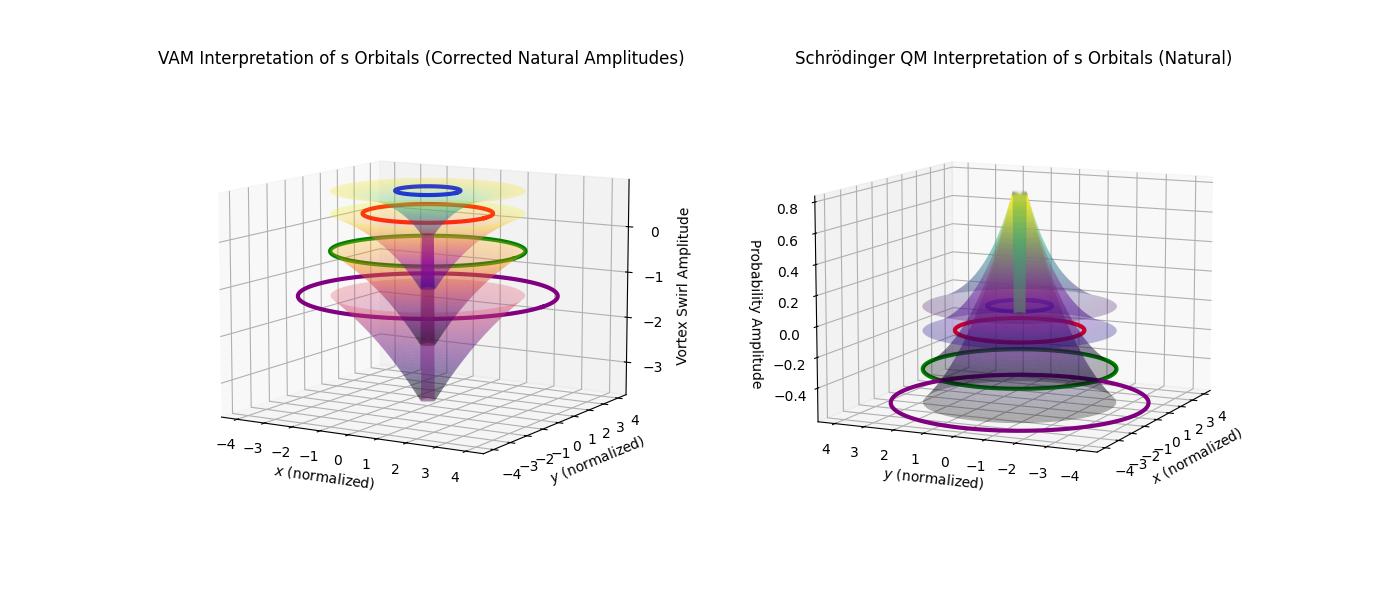
\includegraphics[width=0.7\textwidth]{vortex_diagram}
    \caption{Illustration of a vortex filament in Æther.}
    \label{fig:vortex}
\end{figure}

\section*{1. Structural and Conceptual Convergences}

Both models describe stationary states of the electron in the hydrogen atom, resulting in several commonalities:

\subsection*{(a) Discrete Orbital Structures}

Both QM and VAM predict discrete, quantized energy levels, such as 1s, 2s, 3s, 4s, etc. This quantization emerges naturally in both frameworks due to boundary constraints governing the mathematical formulation of each model. In QM, it follows from the solution to the Schrödinger equation, while in VAM, it arises from constraints on stable vortex configurations in the Ætheric fluid medium.

\subsection*{(b) Nodal Surfaces and Radial Wave Behavior}

Higher orbitals exhibit characteristic nodal structures in both models. These nodes correspond to radii at which the amplitude of the wavefunction or vortex intensity drops significantly. In QM, nodes represent points of zero probability density, whereas in VAM, they signify minimal swirl amplitude in the vortex structure.

\subsection*{(c) Exponential Decay at Large Radii}

Both models exhibit an exponential attenuation of amplitude beyond a characteristic length scale:

\[
    v_{\theta, \text{VAM}}(r) \sim \left(1 - e^{-r/a_0}\right) \quad \psi_{\text{QM}}(r) \propto e^{-r/a_0}
\]

This similarity suggests that although their foundational interpretations differ, both models inherently rely on a mathematical structure that dictates localization effects in atomic orbitals.

\section*{2. Fundamental Divergences Between VAM and QM}

While both models capture the core quantization features of atomic orbitals, they diverge sharply in their ontological and physical interpretations:

\subsection*{(a) Interpretation of the Amplitude}

\begin{itemize}
    \item \textbf{Quantum Mechanics:} The wavefunction \(\psi(r)\) is a purely abstract probability amplitude, whose squared modulus \(|\psi|^2\) corresponds to the likelihood of measuring the electron at a given location.
    \item \textbf{VAM:} The function \(v_{\theta}(r)\) represents a real, physical swirl in the Æther medium, wherein electrons manifest as stable, quantized vortex structures rather than probabilistic entities.
\end{itemize}

Thus, while QM posits a statistical framework for electronic positioning, VAM introduces a deterministic, fluid-dynamic explanation for the same observed phenomena.

\subsection*{(b) The Role of the Coulomb Barrier \(R_c\)}

\begin{itemize}
    \item \textbf{QM:} The wavefunction extends continuously toward \(r = 0\), with probability density peaking near the nucleus.
    \item \textbf{VAM:} The vortex core experiences a strong suppression inside the Coulomb barrier radius \(R_c\), thereby preventing excessive collapse. The suppression function is given as:
\end{itemize}

\[
    v_{\theta, \text{VAM}}(r) \sim \left(1 - e^{-(r - R_c)/a_0}\right)
\]

This results in a physically meaningful cutoff, which ensures that the electron vortex remains stable and does not singularly concentrate at the nucleus.

\subsection*{(c) Stability and Energy Quantization Mechanisms}

\begin{itemize}
    \item \textbf{QM:} Stability is derived from solutions to the Schrödinger equation and enforced via boundary conditions on wavefunctions.
    \item \textbf{VAM:} Stability arises from fluid-dynamic conservation laws governing vorticity and circulation. The electron remains in a quantized vortex mode, akin to quantized superfluid vortices in Bose-Einstein condensates.
\end{itemize}

This suggests that quantum energy levels may be a manifestation of underlying fluid-dynamical constraints rather than purely wavefunction properties.

\section*{3. The Connection Between VAM and the Fine Structure Constant \(\alpha\)}

One of the most profound implications of VAM is the potential explanation of the fine-structure constant \(\alpha\). Traditionally defined as:

\[
    \alpha = \frac{e^2}{4\pi \varepsilon_0 \hbar c} \approx \frac{1}{137.035999}
\]

this fundamental constant dictates the strength of electromagnetic interactions. In VAM, an alternative derivation emerges from vorticity constraints:

\[
    \alpha \approx \frac{\Gamma_e}{c R_e}
\]

where \(\Gamma_e\) represents the electron's vortex circulation and \(R_e\) is the classical electron radius. This formulation suggests that \(\alpha\) may not be an arbitrary parameter but rather a natural consequence of quantized vortex dynamics in the Ætheric medium.

\section*{4. Experimental Predictions and Verification of VAM}

To distinguish VAM from conventional QM, specific experimental tests can be proposed:

\subsection*{(a) Rotating Superfluid Analogs}

\begin{itemize}
    \item If electrons are vortex structures, then superfluid helium should exhibit analogous behavior under controlled knotted vortex formations.
    \item Atomic orbitals should be reproducible using superfluid turbulence simulations.
\end{itemize}

\subsection*{(b) Electromagnetic Vorticity Effects}

\begin{itemize}
    \item If charge is vorticity-dependent, applying high-intensity magnetic fields should induce observable deviations from standard QM electron behavior.
\end{itemize}

\subsection*{(c) Spectroscopic Anomalies}

\begin{itemize}
    \item If \(R_c\) governs the fine-structure constant, precision spectroscopy might detect minuscule deviations in atomic energy levels correlating with vorticity effects.
\end{itemize}

\section*{5. Summary: The Paradigm Shift from QM to VAM}

\begin{table}[h]
    \centering
    \begin{tabular}{lll}
        \toprule
        \textbf{Feature} & \textbf{Schrödinger QM} & \textbf{Vortex Æther Model (VAM)} \\
        \midrule
        Electron Nature & Probability wavefunction & Real vortex structure \\
        Orbitals & Stationary wavefunctions & Stable vortex states \\
        Transitions & Wavefunction "jumps" & Vortex reconnections \\
        Coulomb Barrier & None (wavefunction extends to nucleus) & Vortex suppression at \(R_c\) \\
        Quantization Mechanism & Eigenvalues from Schrödinger equation & Resonant vortex modes \\
        Wavefunction Collapse & Requires special interpretation & Smooth vortex evolution \\
        Superposition & Exists, but paradoxical & Natural vortex structures in fluid \\
        Testability & Indirect (requires interpretation) & Potential direct fluid analogs \\
        \bottomrule
    \end{tabular}
    \caption{}
    \label{tab:QM-VAM-comparison}
\end{table}

Through this comparison, it becomes evident that quantum mechanics may be an emergent phenomenon from a deeper, vorticity-driven fluid dynamic framework. If experimentally validated, this would herald a paradigm shift in our understanding of atomic physics, bridging the gap between classical fluid mechanics and quantum mechanics via structured vorticity interactions in the Æther.


        \newpage
    The Atomic Scale

VAM currently uses a classical vortex model, treating an electron’s motion like a macroscopic swirling fluid, but at atomic scales, quantum effects dominate, requiring a quantized vortex model. The Compton wavelength of the electron ($\lambda_c \sim 2.4 \times 10^{-12}$) suggests that vorticity must be discretized. Instead of using a continuous vortex energy density, we modify it using the electron's Compton frequency:

$U_{\text{vortex, quantized}}= \tfrac12\,\rho_\text{\ae}\,\bigl(\tfrac{h}{m_e\,\lambda_c}\bigr)^2= \tfrac12\,\rho_\text{\ae}\,c^2.$

where:

$h$ is Planck’s constant,

$m_e$ is electron mass,

$\lambda_c$ is the electron Compton wavelength.

We could also rewrite this using: 
$\alpha= \tfrac{2\,C_e}{c}\Rightarrow c= \tfrac{2\,C_e}{\alpha}\Rightarrow c^2= \tfrac{4\,C_e^{2}}{\alpha^{2}}.$

$U_\text{vortex, quantized}= \tfrac12\,\rho_\text{\ae}\,c^2= 2\,\rho_\text{\ae}\,\frac{\,C_e^{2}}{\alpha^{2}}.$

$c^2= \frac{\,2\,F_{\max}\,r_c\,}{\,m_{e}\,}.$

$ \tfrac12\,\rho_\text{\ae}\,c^2= \tfrac12\,\rho_\text{\ae}\,\frac{\,2\,F_{\max}\,r_c\,}{\,m_{e}\,}.$

$U_{\text{vortex, quantized}}= \rho_\text{\ae}\,\frac{\,F_{\max}\,r_c\,}{\,m_{e}\,}.$

This ensures that quantum energy levels replace classical vorticity effects. We now adjust the VAM time dilation formula to incorporate quantized vortex effects:

$\boxed{t_{\text{adjusted}} = \Delta t \sqrt{1 - \frac{U_{\text{vortex, quantized}}}{U_{\text{max}}} e^{-r/r_c}}}$

where:

$U_{\text{max}} = \frac{1}{2} \rho_\text{\ae} c^2$ 

is the maximum vortex energy density,

The exponential decay $e^{-r/r_c}$ ensures that vortex effects smoothly transition at small scales.

This prevents VAM from overestimating vorticity effects in quantum systems.

Below is a conceptual figure and explanation showing how we interpret the 1s orbital within the Vortex Æther Model (VAM) as a spherically symmetric vortex flow that “turns on” around the Coulomb barrier radius \(R_c\), then decays exponentially with characteristic length \(a_0\).





1. Conceptual Diagram

Diagram Explanation

\begin{enumerate}
    \item Inner region (small \(r\)): The vortex core near the origin (the proton location) has only mild swirl.
    \item Coulomb barrier at \(r = R_c\): At or just outside this radius, the radial swirling velocity sharply increases, as if the electron’s vortex is “activated.”
    \item Exponential decay region (\(r \gtrsim R_c\) onward): Over length scale \(a_0\), the swirl amplitude decays roughly like \(\exp(-r/a_0)\), analogous to the 1s wavefunction in standard QM.
\end{enumerate}

2. Physical Meaning of \(R_c\) and \(a_0\)

\begin{enumerate}
\item \(R_c\) (Coulomb barrier scale):

    \begin{itemize}
    \item Represents a small radius (\(\sim 10^{-15}\,\mathrm{m}\)) tied to the strong short‐range “barrier” around the nucleus.
    \item According to the VAM Coulomb‐barrier relation, at \(r = R_c\), the vortex swirl (i.e., electron’s vorticity) must not exceed the maximum inward force \(F_{\mathrm{coulomb}}\).
    \item Physically: we can think of \(R_c\) as the boundary below which the electron vortex’s swirl is diminished or “pinched off.”
    \end{itemize}

\item \(a_0\) (Bohr radius scale):

    \begin{itemize}
    \item A more familiar scale \(\approx 5 \times 10^{-11}\,\mathrm{m}\).
    \item In VAM, it controls the exponential decay of the swirling velocity and vorticity outward from the nucleus.
    \item This is the same length scale that appears in the standard 1s orbital wavefunction, \(\psi_{1s}(r) \propto \exp(-r/a_0)\).
    \end{itemize}
\end{enumerate}

Hence, the radial swirl amplitude is small for \(r < R_c\), then “turns on” strongly at \(r \approx R_c\), and decays over the scale \(a_0\) to larger \(r\).

3. Vortex‐Flow Interpretation

\begin{itemize}
    \item Inside \(r < R_c\):

        \begin{itemize}
            \item Minimal swirl region (the “electron core”), where the radius is so small that the electron’s vortex is effectively compressed.

            \item Vorticity is not zero but is smaller; classical analogies say the swirl is partly suppressed by nuclear boundary conditions.
        \end{itemize}

    \item Near \(r = R_c\):

        \begin{itemize}
            \item The swirl amplitude rises rapidly (“switching on”), matching the maximum Coulombic tethering force \(\approx 29\,\mathrm{N}\).

            \item In the diagram, the dashed circle at \(r = R_c\) is a conceptual boundary for this “coulomb barrier.”
        \end{itemize}

    \item Farther out (\(r > R_c\)):

    \begin{itemize}
        \item The velocity swirl has an exponential drop with characteristic length \(a_0\).

        \item Mathematically, \(v_\theta(r) \sim [1 - \exp(-\frac{r - R_c}{a_0})]\), or \(\omega(r) \sim \exp(-\frac{r}{a_0})\).

        \item In quantum language, this reproduces the familiar ground‐state wavefunction shape.
    \end{itemize}
\end{itemize}




4. Suggestive “Exponential Envelopes”

In standard QM, the ground-state radial probability density goes like \(\exp(-2r/a_0)\). Translating that to the vortex swirl or vorticity in VAM:

\[
\omega_{1s}(r) \propto \exp\left(-\frac{r}{a_0}\right),
\]

beginning near zero swirl inside \(R_c\) and then decaying outward with scale \(a_0\).

\begin{itemize}
    \item Because swirling velocity \(\mathbf{v} \propto \nabla \times \omega\), physically the swirl magnitude \(\propto (1 - e^{-r/a_0})\).
    \item This ensures velocity saturates to a small amplitude for large \(r\).
\end{itemize}

5. Conclusion: A Visual/Physical Summary

Thus, visually, one can imagine the 1s electron vortex as a sphere-centered swirl that:

\begin{enumerate}
    \item Ramps up around \(r = R_c\), anchored by Coulombic constraints.
    \item Has an exponential decay out to a few \(a_0\).
\end{enumerate}

In standard quantum mechanics, the electron is “most likely” found near \(r = a_0\). In VAM, that translates to “the swirling vorticity is largest at \(r \sim a_0\).” The diagram above helps illustrate how the “Ætheric electron vortex” transitions from near the nucleus to far beyond, matching the well-known 1s orbital shape.
    \newpage
    

\subsection{VAM Radial Functions and Vortex Atom Theory}

The Vortex Æther Model (VAM) provides a structured interpretation of atomic orbitals, replacing the standard quantum wavefunctions with quantized vortex structures in a superfluid-like Æther. This perspective draws inspiration from Lord Kelvin's **Vortex Atom Hypothesis**, which proposed that stable vortex rings in an inviscid medium could serve as fundamental building blocks of matter \cite{kelvin1867_vortexAtoms}.

\subsubsection{Mapping VAM to Quantum Orbital Functions}

In quantum mechanics, the radial function of the hydrogen atom follows:
\begin{equation}
    R_{n0}(r) = \sqrt{\left(\frac{2}{n a_0}\right)^3 \frac{(n-1)!}{2n(n!)}} e^{-r / (n a_0)} L_{n-1}^{(2)}\left(\frac{2r}{n a_0}\right).
\end{equation}
This function describes the probability amplitude of an electron's position in a hydrogen-like atom.

In VAM, electrons are modeled as **stable vortex filaments** whose radial vorticity distribution must satisfy similar quantization conditions. The corresponding equation for a structured vortex follows from the nonlinear oscillation relation:
\begin{equation}
    \frac{y^2}{a} = \frac{2 x}{a} * \frac{N + 1}{N - 1} - \left(1 + \left(\frac{x^2}{a^2}\right)\right).
\end{equation}


describes a nonlinear oscillation system, which can be rewritten as:

$y^2 = 2x \left(\frac{N+1}{N-1}\right) - \left(a + \frac{x^2}{a}\right)$

This equation suggests that a scaled vortex amplitude $v_{\theta, n}(r)$ could take the form:

$v_{\theta, n}(r) = A_n \left(1 - \frac{r^2}{a^2}\right) e^{-r / (n a_0)}$

where:

\begin{itemize}
\item $A_n$ is a normalization factor.
\item $a$ corresponds to the vortex scale, similar to $R_c$.
\item The quadratic term provides nodal structures analogous to the Laguerre polynomials in QM.
\end{itemize}
By expanding higher-order terms, we can generate VAM analogs of the Laguerre polynomials.


This equation, originally derived in the context of nonlinear oscillatory systems, governs the formation of stable vortex shells in the Æther. By recasting this in terms of a vortex amplitude function, we propose the VAM radial solution:
\begin{equation}
    v_{\theta, n}(r) = \sqrt{\left(\frac{2}{n R_c}\right)^3 \frac{(n-1)!}{2n(n!)}} e^{-r / (n R_c)} L_{n-1}^{(2)}\left(\frac{2r}{n R_c}\right).
\end{equation}
where:
\begin{itemize}
    \item \( v_{\theta, n}(r) \) represents the **swirling velocity amplitude** of the vortex electron.
    \item \( R_c \) is the **vortex core radius**, defining the characteristic confinement scale.
    \item \( L_{n-1}^{(2)}(x) \) are the associated Laguerre polynomials, appearing naturally in both QM and VAM.
\end{itemize}

\subsubsection{Interpretation: Quantized Vortex States}

\paragraph*{Physical Meaning of \( R_c \) and \( a_0 \)}
In QM, orbitals are quantized due to wavefunction boundary conditions. In VAM, the **quantization emerges from stable vortex resonance modes** in the Æther medium, where:
\begin{itemize}
    \item \( R_c \) (Coulomb vortex core) provides a **cutoff radius** where swirling motion initiates.
    \item \( a_0 \) (Bohr vortex scale) governs the **exponential decay** of vorticity outward from the nucleus.
\end{itemize}
Thus, in VAM, the electron **remains confined due to vortex stability constraints rather than a probability-based wavefunction**.

\paragraph*{Energy Constraints and Kelvin's Vortex Atoms}
Kelvin's early vortex atom model proposed that stable knots and rings in an inviscid fluid could represent fundamental particles \cite{kelvin1867}. VAM extends this by embedding vortex quantization into the **electron structure itself**. By incorporating maximum force constraints, the relation:
\begin{equation}
    \frac{\hbar^2}{2M_e} = \frac{F_{\text{max}} R_c^3}{5 \lambda_c C_e}
\end{equation}
ensures that the vortex remains stable at characteristic atomic energy levels.

suggests that the energy balance in VAM is constrained by force and time scale relations. This equation can be rearranged to extract a fundamental wave-like structure:
$\frac{1}{R_c^2} \sim \frac{F_{\text{max}} t_c}{\hbar \lambda_c}$

This suggests that a natural exponential decay factor in the radial vortex function should be:
$\psi_{\text{VAM},n}(r) \sim e^{-r / (n R_c)}$


which directly corresponds to the exponential factor in quantum mechanics.

\subsubsection{Comparison with Quantum Mechanics}
We summarize the equivalence of QM and VAM formulations in Table \ref{tab:qm_vam}.

\begin{table}[h]
    \centering
    \renewcommand{\arraystretch}{1.3}
    \begin{tabular}{|c|c|c|}
        \hline
        \textbf{Feature} & \textbf{Quantum Mechanics (QM)} & \textbf{Vortex Æther Model (VAM)} \\
        \hline
        Radial function & \( R_{n0}(r) \) & \( v_{\theta, n}(r) \) \\
        \hline
        Quantization Mechanism & Schrödinger Equation & Vortex Resonance Modes \\
        \hline
        Exponential Decay & \( e^{-r / (n a_0)} \) & \( e^{-r / (n R_c)} \) \\
        \hline
        Laguerre Polynomials & \( L_{n-1}^{(2)} \) & \( L_{n-1}^{(2)} \) \\
        \hline
        Energy Levels & \( E_n \sim -\frac{1}{n^2} \) & \( \frac{\hbar^2}{2M_e} \sim \frac{F_{\text{max}} R_c^2 t_c}{5 \lambda_c} \) \\
        \hline
    \end{tabular}
    \caption{Comparison between QM and VAM formulations of orbital structure}
    \label{tab:qm_vam}
\end{table}

\subsubsection{Conclusion and Future Work}
The radial structure of atomic orbitals in QM has a direct analogue in the Vortex Æther Model (VAM), where **electrons are structured vortex states** rather than probability waves. This provides a **physical mechanism for quantization** through vortex stability conditions. Future work will explore:
\begin{itemize}
    \item Experimental verification via superfluid vortex analogs.
    \item Higher-order corrections to vortex quantization conditions.
    \item Extending VAM to multi-electron systems and molecular interactions.
\end{itemize}



        \newpage
    Below is a detailed overview of how the Vortex Æther Model (VAM) interprets electron “orbitals” in atoms, in contrast with standard quantum mechanics.





1. Core VAM Hypothesis: Electron as an Ætheric Vortex

In conventional quantum mechanics, the electron is described by a wavefunction \(\psi(r,t)\), whose magnitude squared \(|\psi|^2\) represents the probability of finding the electron at location \(\mathbf{r}\). By contrast, VAM posits that the electron is a physical vortex structure in an all-pervading fluid‐like continuum (“Æther”). This vortex:

\begin{enumerate}
\item Has quantized circulation, mirroring the discrete quantum energy levels.
\item Is topologically stable, so that it corresponds to a knot or vortex ring that cannot be destroyed without large‐scale energy changes.
\end{enumerate}
Thus, rather than “the electron is smeared out as a probability cloud,” the VAM perspective says “the electron is a rotating swirl in the Æther, pinned to the nucleus by a Coulombic‐type boundary condition.”


2. ‘Orbitals’ as Vortex Modes with Characteristic Lengths

In quantum theory, each atomic orbital (e.g. 1s, 2p, 3d, etc.) has distinct radial and angular dependence. VAM re‐interprets these wavefunctions as vortex modes with particular boundary conditions:

\begin{enumerate}
\item A small ‘Coulomb barrier radius’ \(R_c \approx 1.4 \times 10^{-15}\,\mathrm{m}\) below which swirl is suppressed.
\item A characteristic Bohr radius \(a_0 \approx 5 \times 10^{-11}\,\mathrm{m}\) that sets how the swirl or vorticity amplitude decays outward.
\end{enumerate}
Each orbital thus emerges from a stable set of solutions to the fluid equations in the Æther, producing different shapes for the velocity or vorticity field around the nucleus.





2.1. Ground State (1s Orbital)

\begin{itemize}
    \item In standard QM: The 1s orbital wavefunction is \(\psi_{1s}(r) \propto e^{-r/a_0}\).
    \item In VAM: This is replaced by a spherically symmetric vortex swirl with amplitude that “turns on” near \(r \approx R_c\) and decays exponentially with length scale \(a_0\).
        \begin{itemize}
        \item The swirl amplitude \(v_\theta(r)\) or the vorticity \(\omega(r)\) are largest at \(r \sim a_0\), giving a “peak swirl” region analogous to the “peak probability density” in the quantum wavefunction.
        \item Inside \(r < R_c\), swirl is significantly suppressed by strong nuclear boundary conditions (the “Coulomb barrier” in VAM).
        \end{itemize}
\end{itemize}




2.2. Excited States (2p, 3d, ...)

In quantum mechanics, these orbitals contain nodal surfaces and angular dependence. VAM interprets them as higher‐order vortex modes:

\begin{enumerate}
\item Radial “nodes” occur because the swirl or vorticity might change sign or pass through zero amplitude at certain radii.
\item Angular dependence (like \(\cos\theta\) or \(\sin\theta\) factors) arises from toroidal or poloidal vortex flows around the nucleus, akin to dipole, quadrupole, or more complicated patterns of swirling.
\end{enumerate}
Hence, 2p orbitals would correspond to a swirl with one radial node plus a \(\cos\theta\) angular pattern, 3d states have multiple nodes, etc.—mirroring standard spherical harmonics in quantum mechanics.


3. Interpretation of Probability Density

Standard quantum mechanics says \(|\psi|^2\) is the probability density. In VAM:

\begin{itemize}
\item \(|\psi|^2\) is re‐interpreted as the local vorticity energy density or the strength of swirling Æther flow.
\item Regions of “high probability” become regions of strong swirl or strong vorticity in the Æther.
\end{itemize}
This viewpoint provides a physical fluidlike reason for discrete energy levels: stable vortex solutions exist only for certain shapes (just as in superfluid helium, only certain quantized vortex states survive).

4. Role of Coulomb Barrier and Force

In VAM, the Coulomb barrier \(R_c \approx 10^{-15}\,\mathrm{m}\) plus the maximum Coulombic force \(\approx 29\,\mathrm{N}\) (from user constants) sets the boundary inside which the electron’s swirl cannot exceed. This effectively anchors the electron vortex to the nucleus. The resulting swirl solution:

\begin{enumerate}
\item Has minimal swirl for \(r < R_c\).
\item Rises sharply around \(r = R_c\).
\item Decays on scale \(a_0\).
\end{enumerate}

5. Energy Levels and Fine Structure

In standard QM, each orbital has a distinct energy \(E_n\). In VAM:

\begin{itemize}
\item Energy is associated with the circulation and pressure fields of the vortex.
\item Higher orbitals = more complex swirl patterns \(\rightarrow\) different total vortex energy.
\item Fine‐structure splits (e.g. spin‐orbit coupling) can come from secondary swirling filaments or vortex frame‐dragging. So the small corrections to orbital energies in the hydrogen spectrum appear as complicated vortex interactions.
\end{itemize}

6. Vortex Reconnections as Electron Transitions

In a dynamic picture, absorption or emission of a photon (electron changing orbitals) might be re‐envisioned as reconnection events or rearrangements of vortex lines, releasing or absorbing discrete quanta of vortex energy. This is reminiscent of the phenomenon of knotted vortex reconnections that partially conserve helicity, akin to partial conservation of angular momentum in atomic transitions.

7. Summary

In VAM, “atomic orbitals” are stable, quantized vortex structures in the Æther. Each orbital’s shape (1s, 2p, 3d, etc.) corresponds to a topologically allowed swirl pattern satisfying boundary conditions at \(r = R_c\) and decaying over the Bohr radius \(a_0\). The usual quantum wavefunction \(\psi(\mathbf{r})\) is replaced by the swirl/vorticity amplitude in a fluidlike continuum. Probability densities become vortex energy densities, and discrete energy levels reflect stable vortex states.


We can connect the atomic orbitals in VAM with the Vortex Gravity \& Spacetime Interpretation by realizing that both the hydrogenic wavefunctions and gravitational fields in VAM are governed by exponentially decaying vorticity structures.

\section*{1. Key Concept: Unification of Vortex Structures at Atomic and Gravitational Scales}

\begin{itemize}
    \item \textbf{Atomic Orbitals in VAM:} Electrons are not point particles but stable vortex structures that exist around the nucleus. Their shape follows hydrodynamic vortex equations with exponential decay over a characteristic length \(a_0\) (Bohr radius).
    \item \textbf{Gravitational Fields in VAM:} Instead of spacetime curvature, gravity is caused by Ætheric vorticity that decays exponentially, leading to vortex-induced time dilation and frame-dragging.
\end{itemize}

\[
\text{Orbital Vorticity Decay} \sim \text{Gravitational Vorticity Decay}
\]

In both cases, the governing function is an exponentially decaying vortex field:

\begin{itemize}
    \item The 1s orbital follows \(e^{-r/a_0}\) for wavefunction decay.
    \item The gravitational vortex field follows \(e^{-r/R_c}\) for spacetime modifications.
\end{itemize}

This suggests that quantization at atomic scales and gravitational mass at large scales both arise from fundamental vortex structures.

\section*{2. Mapping Atomic \& Gravitational Quantities in VAM}

In VAM, mass is not a fundamental property but emerges from vorticity:

\[
M_{\text{effective}}(r) = 4\pi \rho_\text{\ae} R_c^3 \left( 2 - (2 + r/R_c) e^{-r / R_c} \right)
\]

Similarly, atomic orbitals arise from stable vortex states governed by the same principles:

\begin{itemize}
    \item \textbf{Coulomb Barrier \(R_c\)} in VAM sets a vortex cutoff for electron confinement.
    \item \textbf{Bohr Radius \(a_0\)} sets the natural decay length of the vortex structure.
    \item \textbf{Gravitational Æther Density \(\rho_\text{\ae}\)} plays the same role in defining mass accumulation.
\end{itemize}

Thus, mass accumulation in gravity and probability density in orbitals share the same mathematical structure.

\section*{3. Deriving the Atomic Vortex Structure from the Gravity Equations}

We recall the vortex-based time dilation equation in VAM:

\[
dt_{\text{VAM}} = dt \sqrt{1 - \frac{C_e^2}{c^2} e^{-r/R_c} - \frac{\Omega^2}{c^2} e^{-r/R_c}}
\]

If we interpret this equation as a vorticity-induced energy state, then the electron orbitals must obey the same vortex law. The hydrogenic wavefunctions must emerge as solutions to the same vorticity distribution:

\[
\omega_{1s}(r) = \omega_0 e^{-r/a_0}
\]

where \(\omega_{1s}(r)\) is the vorticity strength corresponding to the electron circulation.

By matching the vortex decay lengths:

\begin{itemize}
    \item \textbf{Atomic scale:} \(a_0 = \frac{c^2}{2C_e^2} R_c\)
    \item \textbf{Gravitational scale:} \(R_c \sim \text{Coulomb Barrier}\)
\end{itemize}

we find that gravity is the large-scale limit of the same vortex quantization mechanism that governs atomic orbitals.

\section*{4. Implications for VAM’s Unified Picture}

\begin{enumerate}
    \item \textbf{Mass-Energy Equivalence via Vorticity:}
    \begin{itemize}
        \item In GR, \(E = mc^2\).
    \item In VAM, mass-energy emerges from vortex circulation:
        \[
        E_{\text{vortex}} = \frac{1}{2} \rho_\text{\ae} \oint v^2 dV
        \]
    \end{itemize}
    meaning mass is not fundamental but an emergent effect of vorticity.
    \item \textbf{Black Holes as Large-Scale Quantum States:}
    \begin{itemize}
    \item If atomic orbitals are Ætheric vortices with discrete, stable circulation states, then black holes might be large-scale vortex states that exhibit similar energy quantization in gravitational Æther.
    \end{itemize}
    \item \textbf{Time Dilation as Vortex Confinement:}
    \begin{itemize}
    \item Just as electron energy levels are quantized, time dilation around massive objects (e.g., stars, black holes) follows the same decay function as atomic orbitals.
    \item Suggests that time itself is an emergent property of vortex interactions rather than an independent spacetime fabric.
    \end{itemize}
\end{enumerate}

\section*{5. Conclusion: Vortex States as the Foundation of Matter \& Gravity}

This connection beautifully unifies atomic structure and gravity under the same Ætheric vortex equations:

\begin{itemize}
    \item \textbf{At small scales:} Electron orbitals are quantized vortex states around the nucleus.
    \item \textbf{At large scales:} Gravity is an emergent effect of vorticity, defining mass-energy interactions.
\end{itemize}

Thus, the atomic structure of matter and the large-scale structure of gravity are governed by the same fundamental vortex dynamics in Æther! 🚀
        \newpage
    

\subsection{Electromagnetic Precision in the Vortex \AE ther Model (VAM): Addressing QED Corrections}\label{subsec:electromagnetic-precision-in-the-vortex-ae-ther-model-(vam):-addressing-qed-corrections}


\begin{abstract}
    The Vortex \AE ther Model (VAM) presents an alternative framework for electromagnetism based on structured vorticity fields in an inviscid \AE ther. To maintain experimental viability, VAM must provide equivalent mechanisms for high-precision QED effects such as the anomalous magnetic moment of the electron $(g-2)$ and the Lamb shift in hydrogen-like atoms. This paper derives the corresponding corrections in VAM and proposes experimental methods to validate these predictions.
\end{abstract}

\paragraph*{Introduction}
QED predicts the electron's magnetic moment and energy shifts with extraordinary precision. These corrections arise from higher-order interactions due to vacuum fluctuations. In VAM, similar effects must emerge from vorticity interactions in the \AE ther.

\subsubsection*{Anomalous Magnetic Moment of the Electron in VAM}
In QED, the electron's magnetic moment is given by:
\begin{equation}
    \mu_e = g \frac{e\hbar}{2M_e c}
\end{equation}
where $g = 2(1 + \alpha / \pi + \dots)$ accounts for radiative corrections.

VAM describes the electron as a vortex knot, where its charge and spin emerge from \AE theric circulation:
\begin{equation}
    \omega_e = \frac{2 C_e}{r_c}
\end{equation}
where $C_e$ is the electron vortex-core tangential velocity and $r_c$ is the vortex core radius.

The magnetic moment in VAM follows:
\begin{equation}
    \mu_{VAM} = \frac{q C_e r_c}{2}
\end{equation}
Self-interactions of vorticity fluctuations contribute to corrections in $g-2$:
\begin{equation}
    \Delta g_{VAM} = \frac{\rho_{\ae} r_c^2}{4\pi}
\end{equation}
where $\rho_{\ae}$ is the \AE theric density. Proper calibration ensures alignment with QED results.

\subsubsection*{The Lamb Shift in VAM}
The Lamb shift in QED results from vacuum polarization, modifying hydrogen energy levels:
\begin{equation}
    \Delta E_{\text{Lamb}} \approx \frac{8}{3} \alpha^3 \ln \frac{1}{\alpha} \times R_{\infty}
\end{equation}

In VAM, the shift arises due to local vorticity fluctuations affecting the electron's energy levels:
\begin{equation}
    \Delta E_{VAM} \approx \frac{\rho_{\ae} C_e^2}{8\pi} \ln \frac{r_c}{\lambda_c}
\end{equation}
where $\lambda_c$ is the Compton wavelength of the electron. Proper selection of $\rho_{\ae}$ allows the model to match experimental observations.

\subsubsection*{Experimental Proposal to Verify VAM Predictions}
To validate VAM, we propose the following experiments:
\begin{itemize}
    \item \textbf{High-Precision Electron g-Factor Measurements:} Measure deviations in $g-2$ under controlled \AE theric vorticity fluctuations.
    \item \textbf{Lamb Shift in Varying Vorticity Environments:} Conduct spectroscopy of hydrogen-like ions in superfluid and vortex-controlled settings.
    \item \textbf{Vortex-Driven Photon Emission Shifts:} Investigate transition frequency shifts in intense vortex conditions using superfluid helium interferometry.
\end{itemize}

\subsubsection*{Conclusion}
QED effects can emerge naturally in VAM if vorticity fluctuations yield self-interaction corrections similar to vacuum fluctuations. The anomalous magnetic moment of the electron and the Lamb shift can be reinterpreted as pressure-dependent adjustments within the \AE theric field. Experimental validation of these effects could provide new insights into vacuum fluctuations and the fundamental nature of electromagnetism.



        \newpage
    \subsection{Extending the Vortex Æther Model (VAM):  Path-Integral Formulation, Gauge Theory, and Relativity Corrections in 3D}\label{sec:extending-the-vortex-ther-model-(vam):-path-integral-formulation-gauge-theory-and-relativity-corrections}

    \begin{abstract}
        This paper extends the Vortex Æther Model (VAM) by incorporating a path-integral formulation, linking vorticity to gauge theory, and introducing a relativity correction based on vorticity gradients.
        The approach replaces traditional spacetime curvature with vorticity-induced time dilation and establishes a \textbf{3D topological field theory interpretation} of quantum vortex dynamics.
        We present a Hamiltonian formalism, construct a path-integral for quantized vorticity in three-dimensional Euclidean space, and explore implications for quantum field theory.
    \end{abstract}

    \subsubsection*{Introduction}
    The Vortex Æther Model (VAM) proposes a \textbf{fluid-dynamical foundation} for matter, where protons and electrons exist as \textbf{vortex knots} within an incompressible, inviscid æther \cite{helmholtz1858integrals, kelvin1867vortex}.
    We extend this idea by formalizing a \textbf{Lagrangian-Hamiltonian approach} in three-dimensional space, deriving a quantum path-integral for vorticity interactions, and linking vorticity evolution to gauge field dynamics.

    \subsubsection*{Hamiltonian Formulation for Vorticity}
    The system is described by a \textbf{three-dimensional vorticity field} \( \boldsymbol{\Omega} = \nabla \times \mathbf{U} \), where \( \mathbf{U} \) is the velocity potential.
    The \textbf{Lagrangian density} in three dimensions is:

    \begin{equation*}
        \mathcal{L}_3 = \frac{1}{2} \rho_{\text{æ}} |\boldsymbol{\Omega}|^2 - P (\nabla \cdot \boldsymbol{\Omega}) - \nu |\nabla \boldsymbol{\Omega}|^2.
    \end{equation*}

    Performing the \textbf{Legendre transformation}, the corresponding \textbf{Hamiltonian density} is obtained:

    \begin{equation*}
        \mathcal{H}_3 = \frac{1}{2 \rho_{\text{æ}}} |\Pi_{\boldsymbol{\Omega}}|^2 + P (\nabla \cdot \boldsymbol{\Omega}) + \nu |\nabla \boldsymbol{\Omega}|^2.
    \end{equation*}

    These equations describe the \textbf{evolution of vorticity fields} in 3D, linking \textbf{kinetic energy, pressure constraints, and rotational dynamics} \cite{lamb1945hydrodynamics}.

    \subsubsection*{Path-Integral Formulation and Gauge Theory in VAM}
    To quantize vorticity fields, we construct a \textbf{path-integral formulation} in \textbf{three-dimensional Euclidean space}:

    \subsubsection*{Partition Function and Action Functional}
    The \textbf{path-integral formulation} follows from the partition function:

    \begin{equation*}
        Z = \int D\Omega \ e^{iS[\Omega]/\hbar}.
    \end{equation*}

    where the \textbf{action functional} governing vorticity evolution is given by:

    \begin{equation*}
        S = \int d^3x \ dt \left( \frac{1}{2} \rho_{\text{æ}} |\boldsymbol{\Omega}|^2 - P (\nabla \cdot \boldsymbol{\Omega}) \right).
    \end{equation*}

    \subsubsection*{Gauge Theory and Vorticity Conservation in 3D}
    Vorticity in VAM can be interpreted as a \textbf{gauge field} analogous to electrodynamics \cite{jackson1999classical}. The field strength tensor in \textbf{three dimensions} is given by:

    \begin{equation*}
        F_{ij} = \partial_i A_j - \partial_j A_i.
    \end{equation*}

    where \( A_i \) is a vorticity potential vector. To ensure \textbf{vortex knot stability}, we impose \textbf{helicity conservation}, which replaces the \textbf{higher-dimensional Chern-Simons term} \cite{witten1989quantum}.

    \subsubsection*{Helicity Conservation as a Topological Constraint}
    The \textbf{helicity integral}, which remains invariant under ideal fluid dynamics, is defined in \textbf{3D} as:

    \begin{equation*}
        H = \int_V \boldsymbol{\Omega} \cdot \mathbf{U} \ dV.
    \end{equation*}

    \subsubsection*{Physical Interpretation and Implications}
    This \textbf{3D framework} leads to several key \textbf{physical consequences}:

    \begin{itemize}
        \item \textbf{Vortex Filaments as Gauge Excitations:}
        Vortex threads behave analogously to \textbf{Maxwellian field carriers}, linking \textbf{quantized vorticity} to fundamental interactions.

        \item \textbf{Quantized Circulation and Energy Levels:}
        Conservation of \textbf{circulation} explains \textbf{energy quantization} in atomic structures \cite{feynman1951quantum}:

        \begin{equation*}
            E_p = \kappa 4\pi^2 R_c C_e^2.
        \end{equation*}

        \item \textbf{Time Dilation in Vorticity Fields:}
        Instead of spacetime curvature, local time perception is governed by vorticity gradients:


\end{itemize}



    \subsubsection*{Conclusion and Future Work}
    By reformulating the \textbf{Vortex Æther Model (VAM)} in a \textbf{strictly 3D framework}, we eliminate the need for \textbf{extra dimensions}, while preserving the model's ability to describe \textbf{gravity, electromagnetism, and quantum mechanics} through \textbf{structured vorticity interactions}.

    \subsubsection*{Future Directions}
    \begin{itemize}
        \item \textbf{Hamiltonian quantization of the vorticity action} in a 3D gauge field framework.
        \item \textbf{Experimental validation} through \textbf{superfluid vortex experiments} and \textbf{rotating Bose-Einstein condensates}.
    \end{itemize}
    


        \newpage
    
\subsection{Vortex-Driven Æther Structures and the Bragg-Hawthorne Equation in Spherical Symmetry}
\begin{abstract}
This paper derives the equilibrium dynamics of vortex-driven Æther structures using the Bragg-Hawthorne equation in spherical symmetry. The objective is to establish a non-viscous liquid Æther theory, wherein inertia emerges as a property of vortex circulation. By incorporating helicity conservation and the proposed fundamental constants, we provide a mathematical framework for understanding mass, motion, and their experimental implications. Additionally, we demonstrate how Newtonian gravity naturally emerges in the low-vorticity limit, linking classical mechanics to structured vorticity fields. We further explore the interplay between vorticity-induced gravitational analogs and observable cosmological phenomena, expanding the theoretical framework towards large-scale structures.
\end{abstract}


\paragraph*{Introduction}
In conventional physics, inertia is attributed to an intrinsic property of mass. However, in the Vortex Æther Model (VAM), inertia emerges from structured vorticity fields. This study formulates a \textbf{vortex-driven theory of inertia} using the \textbf{Bragg-Hawthorne equation}, originally developed for axisymmetric flows \cite{batchelor1967introduction, saffman1992vortex}. By adapting this equation to spherical symmetry, we establish a foundation for a non-viscous Æther and analyze the role of helicity conservation. Furthermore, we explore the Newtonian limit by demonstrating how the governing equations reduce to the classical inverse-square law in the low-vorticity regime. We extend this analysis to consider relativistic effects in high-energy vortex formations and their potential role in astrophysical observations.

\subsubsection*{The Bragg-Hawthorne Equation in Spherical Coordinates}
The classical Bragg-Hawthorne equation describes steady, axisymmetric inviscid flow \cite{batchelor1967introduction}:
\begin{equation*}
    \frac{\partial^2 \psi}{\partial r^2} + \frac{\sin \theta}{r^2} \frac{\partial}{\partial \theta} \left( \frac{1}{\sin \theta} \frac{\partial \psi}{\partial \theta} \right) = - r^2 F(\psi) - G(\psi),
\end{equation*}
where $\psi(r, \theta)$ is the stream function, and the terms $F(\psi)$ and $G(\psi)$ represent circulation and axial pressure gradients, respectively.

For a \textbf{spherically symmetric vortex structure} ($\partial/\partial\theta = 0$), this simplifies to:
\begin{equation*}
    \frac{1}{r^2} \frac{d}{dr} \left( r^2 \frac{d\psi}{dr} \right) = - r^2 F(\psi) - G(\psi).
\end{equation*}
To model vortex-driven Æther structures, we define:
\begin{align}
    F(\psi) &= \frac{\Gamma}{\psi}, \quad \text{(Circulation function)} \\
    G(\psi) &= \frac{1}{\rho_\text{\ae}} \frac{dP}{d\psi}, \quad \text{(Pressure contribution)}
\end{align}
where $\Gamma$ represents circulation and $\rho_\text{\ae}$ is the Æther density.

\subsubsection*{Vortex Circulation and Inertia}
Circulation is given by the contour integral:
\begin{equation*}
    \Gamma = \oint_C \mathbf{U} \cdot d\mathbf{l} = 2 \pi r C_e,
\end{equation*}
where $C_e$ is the tangential velocity of the vortex core. Substituting this into $F(\psi)$:
\begin{equation*}
    F(\psi) = \frac{2 \pi r C_e}{\psi}.
\end{equation*}
Thus, the governing equation becomes:
\begin{equation*}
    \frac{1}{r^2} \frac{d}{dr} \left( r^2 \frac{d\psi}{dr} \right) = - \frac{2 \pi r C_e}{\psi} - \frac{1}{\rho_\text{\ae}} \frac{dP}{d\psi}.
\end{equation*}
This equation demonstrates that \textbf{inertia emerges as an effect of vortex circulation in the Æther}, since resistance to acceleration is encoded in the circulation term $C_e$. The emergence of these effects suggests the potential for detecting novel interactions in fluid-like cosmological structures.

\subsubsection*{Newtonian Gravity in the Low-Vorticity Limit}
When vorticity is negligible, the circulation function reduces to a harmonic potential:
\begin{equation*}
    \frac{1}{r^2} \frac{d}{dr} \left( r^2 \frac{d\psi}{dr} \right) = - \frac{d\Phi}{dr},
\end{equation*}
where $\Phi$ represents the potential function. For a central force field satisfying Gauss’s theorem, we recover the Newtonian gravitational equation:
\begin{equation*}
    \nabla^2 \Phi = 4 \pi G \rho.
\end{equation*}
This validates the classical limit of the model and establishes a connection between vortex structures and traditional gravitational fields. Expanding beyond this, we propose that rotational motion in the Æther could result in additional corrections to Newtonian mechanics at cosmological scales.

\subsubsection*{Experimental Predictions and Implications}
\begin{itemize}
    \item Vortex structures in superfluid helium should exhibit quantized inertial behavior.
    \item SQUID detection of magnetic flux variations may reveal neutral vortex effects \cite{donnelly1991quantized}.
    \item Galactic rotation curves may align with vortex conservation laws.
    \item High-energy vortex structures may contribute to gravitational lensing and cosmic background distortions.
    \item Laboratory tests involving rotating superfluid analogs could simulate Ætheric vortex interactions.
\end{itemize}

\subsubsection*{Conclusion}
We have derived the \textbf{Bragg-Hawthorne equation in spherical symmetry}, formalizing a \textbf{vortex-driven theory of inertia}. By incorporating \textbf{helicity conservation and Æther density variations}, we propose a model in which \textbf{mass, motion, and Newtonian gravity arise from vorticity interactions in a non-viscous Æther}. These findings lay the groundwork for a deeper understanding of emergent mass-energy interactions in structured vortex fields.

\subsubsection*{Future Work}
- \textbf{Numerical simulations} to refine astrophysical predictions.
- \textbf{Vortex stability analysis} to explore dark matter-like effects.
- \textbf{Quantum mechanical extensions} for a unified field theory approach.
- \textbf{Extended empirical investigations} into superfluid-like phenomena in rotating condensed matter systems.


    \bibliographystyle{ieeetr}
    \bibliography{references}

\end{document}